

\documentclass[conference]{IEEEtran}
% Some Computer Society conferences also require the compsoc mode option,
% but others use the standard conference format.
%
% If IEEEtran.cls has not been installed into the LaTeX system files,
% manually specify the path to it like:
% \documentclass[conference]{../sty/IEEEtran}





% Some very useful LaTeX packages include:
% (uncomment the ones you want to load)


% *** MISC UTILITY PACKAGES ***
%
%\usepackage{ifpdf}
% Heiko Oberdiek's ifpdf.sty is very useful if you need conditional
% compilation based on whether the output is pdf or dvi.
% usage:
% \ifpdf
%   % pdf code
% \else
%   % dvi code
% \fi
% The latest version of ifpdf.sty can be obtained from:
% http://www.ctan.org/pkg/ifpdf
% Also, note that IEEEtran.cls V1.7 and later provides a builtin
% \ifCLASSINFOpdf conditional that works the same way.
% When switching from latex to pdflatex and vice-versa, the compiler may
% have to be run twice to clear warning/error messages.






% *** CITATION PACKAGES ***
%
%\usepackage{cite}
% cite.sty was written by Donald Arseneau
% V1.6 and later of IEEEtran pre-defines the format of the cite.sty package
% \cite{} output to follow that of the IEEE. Loading the cite package will
% result in citation numbers being automatically sorted and properly
% "compressed/ranged". e.g., [1], [9], [2], [7], [5], [6] without using
% cite.sty will become [1], [2], [5]--[7], [9] using cite.sty. cite.sty's
% \cite will automatically add leading space, if needed. Use cite.sty's
% noadjust option (cite.sty V3.8 and later) if you want to turn this off
% such as if a citation ever needs to be enclosed in parenthesis.
% cite.sty is already installed on most LaTeX systems. Be sure and use
% version 5.0 (2009-03-20) and later if using hyperref.sty.
% The latest version can be obtained at:
% http://www.ctan.org/pkg/cite
% The documentation is contained in the cite.sty file itself.






% *** GRAPHICS RELATED PACKAGES ***
%
\ifCLASSINFOpdf
   \usepackage[pdftex]{graphicx}
  % declare the path(s) where your graphic files are
  % \graphicspath{{../pdf/}{../jpeg/}}
  % and their extensions so you won't have to specify these with
  % every instance of \includegraphics
   \DeclareGraphicsExtensions{.pdf,.jpeg,.png}
\else
  % or other class option (dvipsone, dvipdf, if not using dvips). graphicx
  % will default to the driver specified in the system graphics.cfg if no
  % driver is specified.
\usepackage[dvips]{graphicx}
  % declare the path(s) where your graphic files are
   \graphicspath{{../eps/}}
  % and their extensions so you won't have to specify these with
  % every instance of \includegraphics
  % \DeclareGraphicsExtensions{.eps}
\fi
% graphicx was written by David Carlisle and Sebastian Rahtz. It is
% required if you want graphics, photos, etc. graphicx.sty is already
% installed on most LaTeX systems. The latest version and documentation
% can be obtained at: 
% http://www.ctan.org/pkg/graphicx
% Another good source of documentation is "Using Imported Graphics in
% LaTeX2e" by Keith Reckdahl which can be found at:
% http://www.ctan.org/pkg/epslatex
%
% latex, and pdflatex in dvi mode, support graphics in encapsulated
% postscript (.eps) format. pdflatex in pdf mode supports graphics
% in .pdf, .jpeg, .png and .mps (metapost) formats. Users should ensure
% that all non-photo figures use a vector format (.eps, .pdf, .mps) and
% not a bitmapped formats (.jpeg, .png). The IEEE frowns on bitmapped formats
% which can result in "jaggedy"/blurry rendering of lines and letters as
% well as large increases in file sizes.
%
% You can find documentation about the pdfTeX application at:
% http://www.tug.org/applications/pdftex





% *** MATH PACKAGES ***
%
%\usepackage{amsmath}
% A popular package from the American Mathematical Society that provides
% many useful and powerful commands for dealing with mathematics.
%
% Note that the amsmath package sets \interdisplaylinepenalty to 10000
% thus preventing page breaks from occurring within multiline equations. Use:
%\interdisplaylinepenalty=2500
% after loading amsmath to restore such page breaks as IEEEtran.cls normally
% does. amsmath.sty is already installed on most LaTeX systems. The latest
% version and documentation can be obtained at:
% http://www.ctan.org/pkg/amsmath





% *** SPECIALIZED LIST PACKAGES ***
%
%\usepackage{algorithmic}
% algorithmic.sty was written by Peter Williams and Rogerio Brito.
% This package provides an algorithmic environment fo describing algorithms.
% You can use the algorithmic environment in-text or within a figure
% environment to provide for a floating algorithm. Do NOT use the algorithm
% floating environment provided by algorithm.sty (by the same authors) or
% algorithm2e.sty (by Christophe Fiorio) as the IEEE does not use dedicated
% algorithm float types and packages that provide these will not provide
% correct IEEE style captions. The latest version and documentation of
% algorithmic.sty can be obtained at:
% http://www.ctan.org/pkg/algorithms
% Also of interest may be the (relatively newer and more customizable)
% algorithmicx.sty package by Szasz Janos:
% http://www.ctan.org/pkg/algorithmicx




% *** ALIGNMENT PACKAGES ***
%
%\usepackage{array}
% Frank Mittelbach's and David Carlisle's array.sty patches and improves
% the standard LaTeX2e array and tabular environments to provide better
% appearance and additional user controls. As the default LaTeX2e table
% generation code is lacking to the point of almost being broken with
% respect to the quality of the end results, all users are strongly
% advised to use an enhanced (at the very least that provided by array.sty)
% set of table tools. array.sty is already installed on most systems. The
% latest version and documentation can be obtained at:
% http://www.ctan.org/pkg/array


% IEEEtran contains the IEEEeqnarray family of commands that can be used to
% generate multiline equations as well as matrices, tables, etc., of high
% quality.




% *** SUBFIGURE PACKAGES ***
%\ifCLASSOPTIONcompsoc
%  \usepackage[caption=false,font=normalsize,labelfont=sf,textfont=sf]{subfig}
%\else
%  \usepackage[caption=false,font=footnotesize]{subfig}
%\fi
% subfig.sty, written by Steven Douglas Cochran, is the modern replacement
% for subfigure.sty, the latter of which is no longer maintained and is
% incompatible with some LaTeX packages including fixltx2e. However,
% subfig.sty requires and automatically loads Axel Sommerfeldt's caption.sty
% which will override IEEEtran.cls' handling of captions and this will result
% in non-IEEE style figure/table captions. To prevent this problem, be sure
% and invoke subfig.sty's "caption=false" package option (available since
% subfig.sty version 1.3, 2005/06/28) as this is will preserve IEEEtran.cls
% handling of captions.
% Note that the Computer Society format requires a larger sans serif font
% than the serif footnote size font used in traditional IEEE formatting
% and thus the need to invoke different subfig.sty package options depending
% on whether compsoc mode has been enabled.
%
% The latest version and documentation of subfig.sty can be obtained at:
% http://www.ctan.org/pkg/subfig




% *** FLOAT PACKAGES ***
%
%\usepackage{fixltx2e}
% fixltx2e, the successor to the earlier fix2col.sty, was written by
% Frank Mittelbach and David Carlisle. This package corrects a few problems
% in the LaTeX2e kernel, the most notable of which is that in current
% LaTeX2e releases, the ordering of single and double column floats is not
% guaranteed to be preserved. Thus, an unpatched LaTeX2e can allow a
% single column figure to be placed prior to an earlier double column
% figure.
% Be aware that LaTeX2e kernels dated 2015 and later have fixltx2e.sty's
% corrections already built into the system in which case a warning will
% be issued if an attempt is made to load fixltx2e.sty as it is no longer
% needed.
% The latest version and documentation can be found at:
% http://www.ctan.org/pkg/fixltx2e


%\usepackage{stfloats}
% stfloats.sty was written by Sigitas Tolusis. This package gives LaTeX2e
% the ability to do double column floats at the bottom of the page as well
% as the top. (e.g., "\begin{figure*}[!b]" is not normally possible in
% LaTeX2e). It also provides a command:
%\fnbelowfloat
% to enable the placement of footnotes below bottom floats (the standard
% LaTeX2e kernel puts them above bottom floats). This is an invasive package
% which rewrites many portions of the LaTeX2e float routines. It may not work
% with other packages that modify the LaTeX2e float routines. The latest
% version and documentation can be obtained at:
% http://www.ctan.org/pkg/stfloats
% Do not use the stfloats baselinefloat ability as the IEEE does not allow
% \baselineskip to stretch. Authors submitting work to the IEEE should note
% that the IEEE rarely uses double column equations and that authors should try
% to avoid such use. Do not be tempted to use the cuted.sty or midfloat.sty
% packages (also by Sigitas Tolusis) as the IEEE does not format its papers in
% such ways.
% Do not attempt to use stfloats with fixltx2e as they are incompatible.
% Instead, use Morten Hogholm'a dblfloatfix which combines the features
% of both fixltx2e and stfloats:
%
% \usepackage{dblfloatfix}
% The latest version can be found at:
% http://www.ctan.org/pkg/dblfloatfix




% *** PDF, URL AND HYPERLINK PACKAGES ***
%
\usepackage{url}
% url.sty was written by Donald Arseneau. It provides better support for
% handling and breaking URLs. url.sty is already installed on most LaTeX
% systems. The latest version and documentation can be obtained at:
% http://www.ctan.org/pkg/url
% Basically, \url{my_url_here}.
\usepackage{hyperref}

\usepackage[T1]{fontenc}
\usepackage{fancyvrb,cprotect}

% correct bad hyphenation here
\hyphenation{op-tical net-works semi-conduc-tor}
\providecommand{\keywords}[1]{\textbf{\textit{Keywords--}} #1}

\begin{document}
%
% paper title
\title{Impact of Refactoring on Source Code: A Computational Linguistics Approach}


% author names and affiliations
% use a multiple column layout for up to three different
% affiliations
\author{\IEEEauthorblockN{Musfiqur Rahman\IEEEauthorrefmark{1},
		Nafiz Islam\IEEEauthorrefmark{2}}
	\IEEEauthorblockA{Department of Computer Science and Software Engineering\\
		Concordia University\\
		Montreal, Canada\\
		Email: \IEEEauthorrefmark{1}musfiqur.rahman@mail.concordia.ca,
		\IEEEauthorrefmark{2}na\_islam@encs.concordia.ca}}

\maketitle

% As a general rule, do not put math, special symbols or citations
% in the abstract
\begin{abstract}
Naturalness is fundamentally repetitiveness or predictability.  Like the natural language, programming languages are natural. Researchers used that idea to improve 
Statistical Models of code, Porting and Translation, Studying the Naural Linguistics of Code, Suggestions and Completions, Analysis and Tools, Assistive Technologies, Corpus Curation etc. Refactored code are simpler, understandable, efficient and compact, so refactored code should be more natural. In this paper, we investigate this hypothesis. We consider a large corpus of smelly data and refactored data from 10 different Java projects, and focus on its language statistics, evaluating the naturalness of smelly code. Initially the smells are refactored using automated tool \textit{JDeodorant} and our results show that the perplexity of refactored data is less than the smelly code. Which indicates that refactored code are more natural than smelly code.
\end{abstract}

% keywords
\keywords{\textbf{Refactoring; code smell; n-gram; language model}}


% For peer review papers, you can put extra information on the cover
% page as needed:
% \ifCLASSOPTIONpeerreview
% \begin{center} \bfseries EDICS Category: 3-BBND \end{center}
% \fi
%
% For peerreview papers, this IEEEtran command inserts a page break and
% creates the second title. It will be ignored for other modes.
\IEEEpeerreviewmaketitle



\section{INTRODUCTION} \label{Intro}

Programming languages show similar pattern in terms of repetitiveness like any natural language. Although programming languages are artificially developed with more compact rules both syntactically and semantically, surprisingly, they are even more predictable and repetitive than natural human languages. This idea was first discussed in \cite{Hindle} where Hindle \textit{et al.} capture the regular and predictable nature of programming languages by \textit{n-gram} language model. Moreover, they use this information captured by the \textit{n-gram} language model in code suggestions. Later on, it was shown by Tu \textit{el al.} \cite{Tu} that by using \textit{cache-based} language model the naturalness can be captured even better as source codes are more repetitive locally (i.e. in file level) than they are repetitive globally (i.e. in the whole project corpus). Using cache-based language model improves the quality of code suggestion task. Besides code suggestion, this idea of repetitiveness of software source code has been exploited in suggesting bug fixes as well \cite{Ray}.

The process in which developers improve the architecture and design of an existing source code without effecting its functionality is known as \textit{Refactoring} \cite{Opdyke}. Refactoring is performed on source code due to various reasons like, adding new features, bug fix requests, code smell etc. \cite{Silva}. Sometimes developers take help of tools to perform refactoring, whereas in most of the cases they put manual effort in doing so \cite{Murphy}\cite{Silva}. Although many of the modern Integrated Development Environments (IDEs) come with the feature of refactoring, researchers are also putting considerable amount of effort in developing tools to automate refactoring \cite{GailMurphy}\cite{Davood}. Over all, the idea of refactoring has become a crucial part of software development nowadays and refactorig has made softwares more maintainable, more reusable and more readable. Threfore, many works have so far been done on theory and applications of refactoring \cite{Zibran}\cite{Mondal}\cite{Fokaefs}\cite{Tsantalis}. This huge amount of application of refactoring in both theory and practice rises an interesting question: \textit{How does refactoring affect the naturalness of source code?}

The effect of refactoring on source code can be studied by using \textit{Language Model} \cite{Brown}. Language modelling is a very popular approach in the field of \textit{Statistical Machine Translation (SMT)} \cite{Koehn} and \textit{Natural Language Processing (NLP)} \cite{Jones}. Previous works that had studied the naturalness of software source code also mathematically defined the term \textbf{naturalness} based on the theory of language modelling \cite{Ray}\cite{Hindle}\cite{Tu}. After being trained on a large corpus language models assign higher naturalness to previously seen code, while assigning lower naturalness to unseen or rarely seen code \cite{Tu}. For example, Campbell \textit{et al.} \cite{Campbell} showed that language models mark code which is syntactically faulty as \textit{unlikely} or \textit{less likely}.

\subsection{Research Questions}
We investigate the impact of refactoring on the naturalness of source code by addressing the following issues:
\begin{itemize}
\item change in naturalness of the code after applying tool-based refactoring
\item change in naturalness of the code after applying manual refactoring
\item different types of refactoring and naturalness of code
\end{itemize}
More specifically we try to answer to following three research questions.

\textit{RQ1. Real refactoring: Does refactoring that developers perform change the cross-entorpy of the source code?}

We determine the naturalness of source code before and after the refactoring has been performed by a developer. We try to find whether the naturalness drops, increases or remains same after performing refactoring.

\textit{RQ2. Tool-based or automated refactoring: Does automated refactoring change the naturalness?}

Like \textit{RQ1}, in \textit{RQ2} also we determine the naturalness of source code before and after the refactoring has been performed. This time the refactoring is done by using tool, and not by the developer. This time also we try to find whether the naturalness drops, increases or remains same after performing refactoring.

\textit{RQ3, Types of refactoring: How do different types of refactoring affect the naturalness?}

There are multiple types of refactoring. We investigate their impact on naturalness separately and try to find how differently (or similarly) different types of refactoring impact the naturalness.

Rest of the paper is structured in the following way. In Section \ref{Methodology} we discuss about the our data source, methodology along with some theoretical background. Three RQ1, RQ2 and RQ3 are discussed in Section III, IV and V respectively. 
% You must have at least 2 lines in the paragraph with the drop letter
% (should never be an issue)
%I wish you the best of success.

%\hfill mds
 
%\hfill August 26, 2015
\section{DATA SOURCE AND METHODOLOGY} \label{Methodology}
% no \IEEEPARstart
\subsection{Data}
Our primary data source is the open-source GitHub projects. For our study, we search for refactorings performed in different versions of the selected repositories. In order to do that we perform analysis on the differences between the source code of the refactored project before and after the refactoring was performed. We use a refactoring detection tool called \textit{RefactoringMiner} \cite{Silva} for accomplishing the analysis task. This tool gives us information about the commit id associated with the refactoring, type of refactoring that has been performed, files that have been changed etc. Thus, we get the two versions of the project: \textit{the version before refactoring} and \textit{the version after refactoring}. Note that \textit{RefactoringMiner} detects refactoring only in the projects written in Java. Furthermore, it cannot yet detect all types of refactoring. For example, the tool cannot detect \textit{RENAME CLASS/METHOD/FIELD} refactoring types. The detailed underlying theory behind how the tool works along with its limitations are discussed in \cite{NikolaosTsantalis}. Summary of our data is shown in Table \ref{SuammaryTable}.



\begin{table*}[t]
\centering
\caption{Summary of the Data}
\label{SuammaryTable}
 \begin{tabular}{||c c c c c c c||} 
 \hline
 Project Name & Type & Access Date & Files (*.java) & Comments & Lines of Code &  \#of tokens \\ [0.5ex] 
 \hline\hline
 Vert.x & Before Refactoring & 20-Jul-2016 & 414 & 21837 & 50436 & 407825 \\ 
 \hline
   & After Manual Refactoring & 20-Jul-2016 & 437 & 21927 & 51920 & 422390 \\
 \hline
 languagetool & Before Refactoring & 18-Jul-2016 & 949 & 27320 & 73045 & 646598 \\
 \hline
   & After Manual Refactoring & 18-Jul-2016 & 949 & 27319 & 73060 & 646691 \\
 \hline
 Aeron & Before Refactoring & 20-Jul-2016 & 237 & 8369 & 26667 & 193956 \\
 \hline
   & After Manual refactoring & 20-Jul-2016 & 237 & 8369 & 26649 & 194053 \\
   \hline
 checkstyle & Before Refactoring & 20-Jul-2016 & 1092 & 39712 & 73214 & 504086 \\
 \hline
   & After Manual Refactoring & 20-Jul-2016 & 1092 & 39695 & 73175 & 503857 \\
   \hline
  Guacamole-client & Before Refactoring & 18-Jul-2016 & 327 & 19558 & 11855 & 90044 \\
  \hline
   & After Manual Refactoring & 18-Jul-2016 & 327 & 19564 & 11859 & 90061 \\ 
  \hline
   processing & Before Refactoring & 20-Jul-2016 & 228 & 50577 & 91024 & 698598 \\
  \hline
  & After Manual Refactoring & 20-Jul-2016 & 228 & 50576 & 91024 & 698603 \\
  \hline
  Buck & Before Refactoring & 23-Jul-2016 & 2269 & 82571 & 226583 & 1966841 \\
  \hline
  & After Manual Refactoring & 23-Jul-2016 & 2271 & 82601 & 226674 & 1967353 \\
  \hline
  orientdb & Before Refactoring & 23-Jul-2016 & 2057 & 55111 & 265440 & 2363105 \\
  \hline
   & After Manual Refactoring & 23-Jul-2016 & 2060 & 55152 & 265664 & 2364702 \\
  \hline
  atomix & Before Refactoring & 23-Jul-2016 & 254 & 13916 & 19424 & 147668 \\
  \hline
    & After Manual Refactoring & 23-Jul-2016 & 254 & 13917 & 19424 & 147623 \\
  \hline
  fabric8 & Before Refactoring & 20-Jul-2016 & 913 & 24045 & 65966 & 531673 \\
   \hline
   & After Manual Refactoring & 20-Jul-2016 & 913 & 24045 & 65953 & 531516 \\ [1ex]  
 \hline
\end{tabular}
\end{table*}

\subsection{Background}

\subsubsection{Language Model}

In this paper, we use the term language model (LM), which is nothing but probability distributions over sequence of \textit{m} tokens \textit{P(k$_1$, k$_2$,..., k$_m$)}. Language Model is trained on a corpus of sequences of tokens from the language, with the goal of assigning high probability to tokens with maximum likelihood, and low probability to tokens with minimum likelihood. Language models are needed to model the uncertainty of the language by determining the most probable sequence of tokens for a given input. 

\subsubsection{N-Gram Language Model}
Consider the sequence of tokens \textit{k$_1$, k$_2$, k$_3$, ... k$_{m-1}$, k$_m$} in a document, \textit{D}. N-gram model statistically calculates likelihood of tokens to follow other tokens. Thus, we can estimate the probability of a document based on the product of a series of conditional probabilities: 
\\
\begin{equation}
P(D) = P(k_1) P(k_2 | k_1) P(k_3 | k_1, k_2) ... P(k_n | k_1, k_2,..., k_{n-1})
\end{equation}
\\
Where \textit{P(D)} is the probability of document and \textit{P(k$_i$)} is the conditional probability of tokens. 
We can transform above equation to following more general form of equation. 
\\
\begin{equation}
P(k_1, k_2, k_3,..., k_{m-1}, k_m) = \sum_{i=1}^{m} P(k_i | k_1,..., k_{n-1})
\end{equation}
In this transformation it is assumed that token occurrences are influenced only by limited prefix of length n. This assumption is known as \textbf{Markov Property} as described by Zhang \textit{et al.} \cite{Zhang}. Furthermore, we can consider this as a Markov Chain which assumes that the outcome of next step depends only on current step. Thus we can write:
\\
\begin{equation}
P(k_i|k_{i-(n-1)},..., k_{i-1})=P(k_i|k_{i-(n-1)})
\end{equation}
\\
To use above equation we need to know conditional probabilities values for each token for each possible n-gram. The conditional probability can be calculated from n-gram frequency counts.

Bigram and Trigram language models can be modeled with value of \textit{n = 2} and \textit{n = 3} respectively. 
\\
\subsubsection{Cross Entropy}

Cross entropy is used to compare probability distributions when the true probability distribution is unknown. Given a corpus \textit{K} of size \textit{N} consisting of tokens k$_1$, k$_2$,..., k$_n$, the log probability of the model distribution \textit{m} with true distribution \textit{p} on this corpus is defined as, 
\\
\begin{equation}
H(P,m) = \sum_{}^{} P(x)log_2(m)(x)
\end{equation}
\textit{H(P,m)} indicates the average number of bits required to encode messages sampled from p with a coding scheme based on \textit{m}.
\\
\textit{H(P)} is a lower bound on \textit{H(P,m)} and \textit{H(P,m)} is an upper bound on \textit{H(P)}. The lower \textit{H(P,m)}, the closer the model \textit{m} is to the truth.\cite {peter} \cite {julia}
\\
\subsubsection{Perplexity}
Perplexity is a per-word average of the probability with which the language model generates the test data set, where the average is over the number of words in the test data set. 
\\
The perplexity of a discrete probability distribution \textit{P} is defined as 
\\
\begin{equation}
2^{H(P)} = 2 - \sum_{}^{} P(x)log _2(P)(x)
\end{equation}
\\where \emph{H(p)} is the entropy of the distribution and \textit{x} ranges over events.

\subsection{Methodology}
\subsubsection{Data Extraction}
After getting the two versions of the source code of the project we extract the files that have been changed. From those source files with extract the lines that have been changed. There are two types of changes:
 \begin{itemize}
 \item Addition: a line is added to the source file
 \item Deletion: a line is removed from the source file
 \end{itemize}
We separately extract added and deleted lines from the two versions of the project. We use {\fontfamily{qcr}\selectfont git-diff} command to extract the changed lines.

\subsubsection{Data Preprocessing} \label{Preprocessing}
For each data set in our hand, we preprocess the data by removing comments from the source file, and then perform lexical analysis according to the language syntax. We use ANTLR4 \footnote{http://www.antlr.org/} to lexicalyze the raw code and generate token sequence.

\subsubsection{Perplexity Calculation}
The sequence of tokens generated in previous step (Section \ref{Preprocessing}) are used to train and test the \textit{n-gram} language model. Each data set (i.e. each version of a project) is divided into two parts of 90\% and 10\% of the preprocessed data. We train our language model on the 90\% portion, and validate the model on the 10\% portion. Results are averaged out over 10-fold cross validation. We use MIT Language Model (MITLM) toolkit \footnote{https://github.com/mitlm/mitlm} for calculating the perplexity of each data set. For our study we use 1 to 10 as the value of \textit{n}.

The logarithm of perplexity is defined as \textit{cross-entropy}, which is the measure of naturalness of the data \cite{Hindle}. \textit{The less the cross-entropy value is, the more natural and predictable the data are.}


\section{Real Refactoring} \label{ReallRefactoring}
\textit{RQ1. Real refactoring: Does refactoring that developers perform change the cross-entorpy of the source code?}


As shown by Silva \textit{et al.} \cite{Silva}, most of the refactorings are done by the developers manually. We try to determine how, if at all, refactoring changes the cross-entropy of the source code by answering to \textit{RQ1}. 

\subsection{Finding}

\begin{figure*}[ht!]
\centering
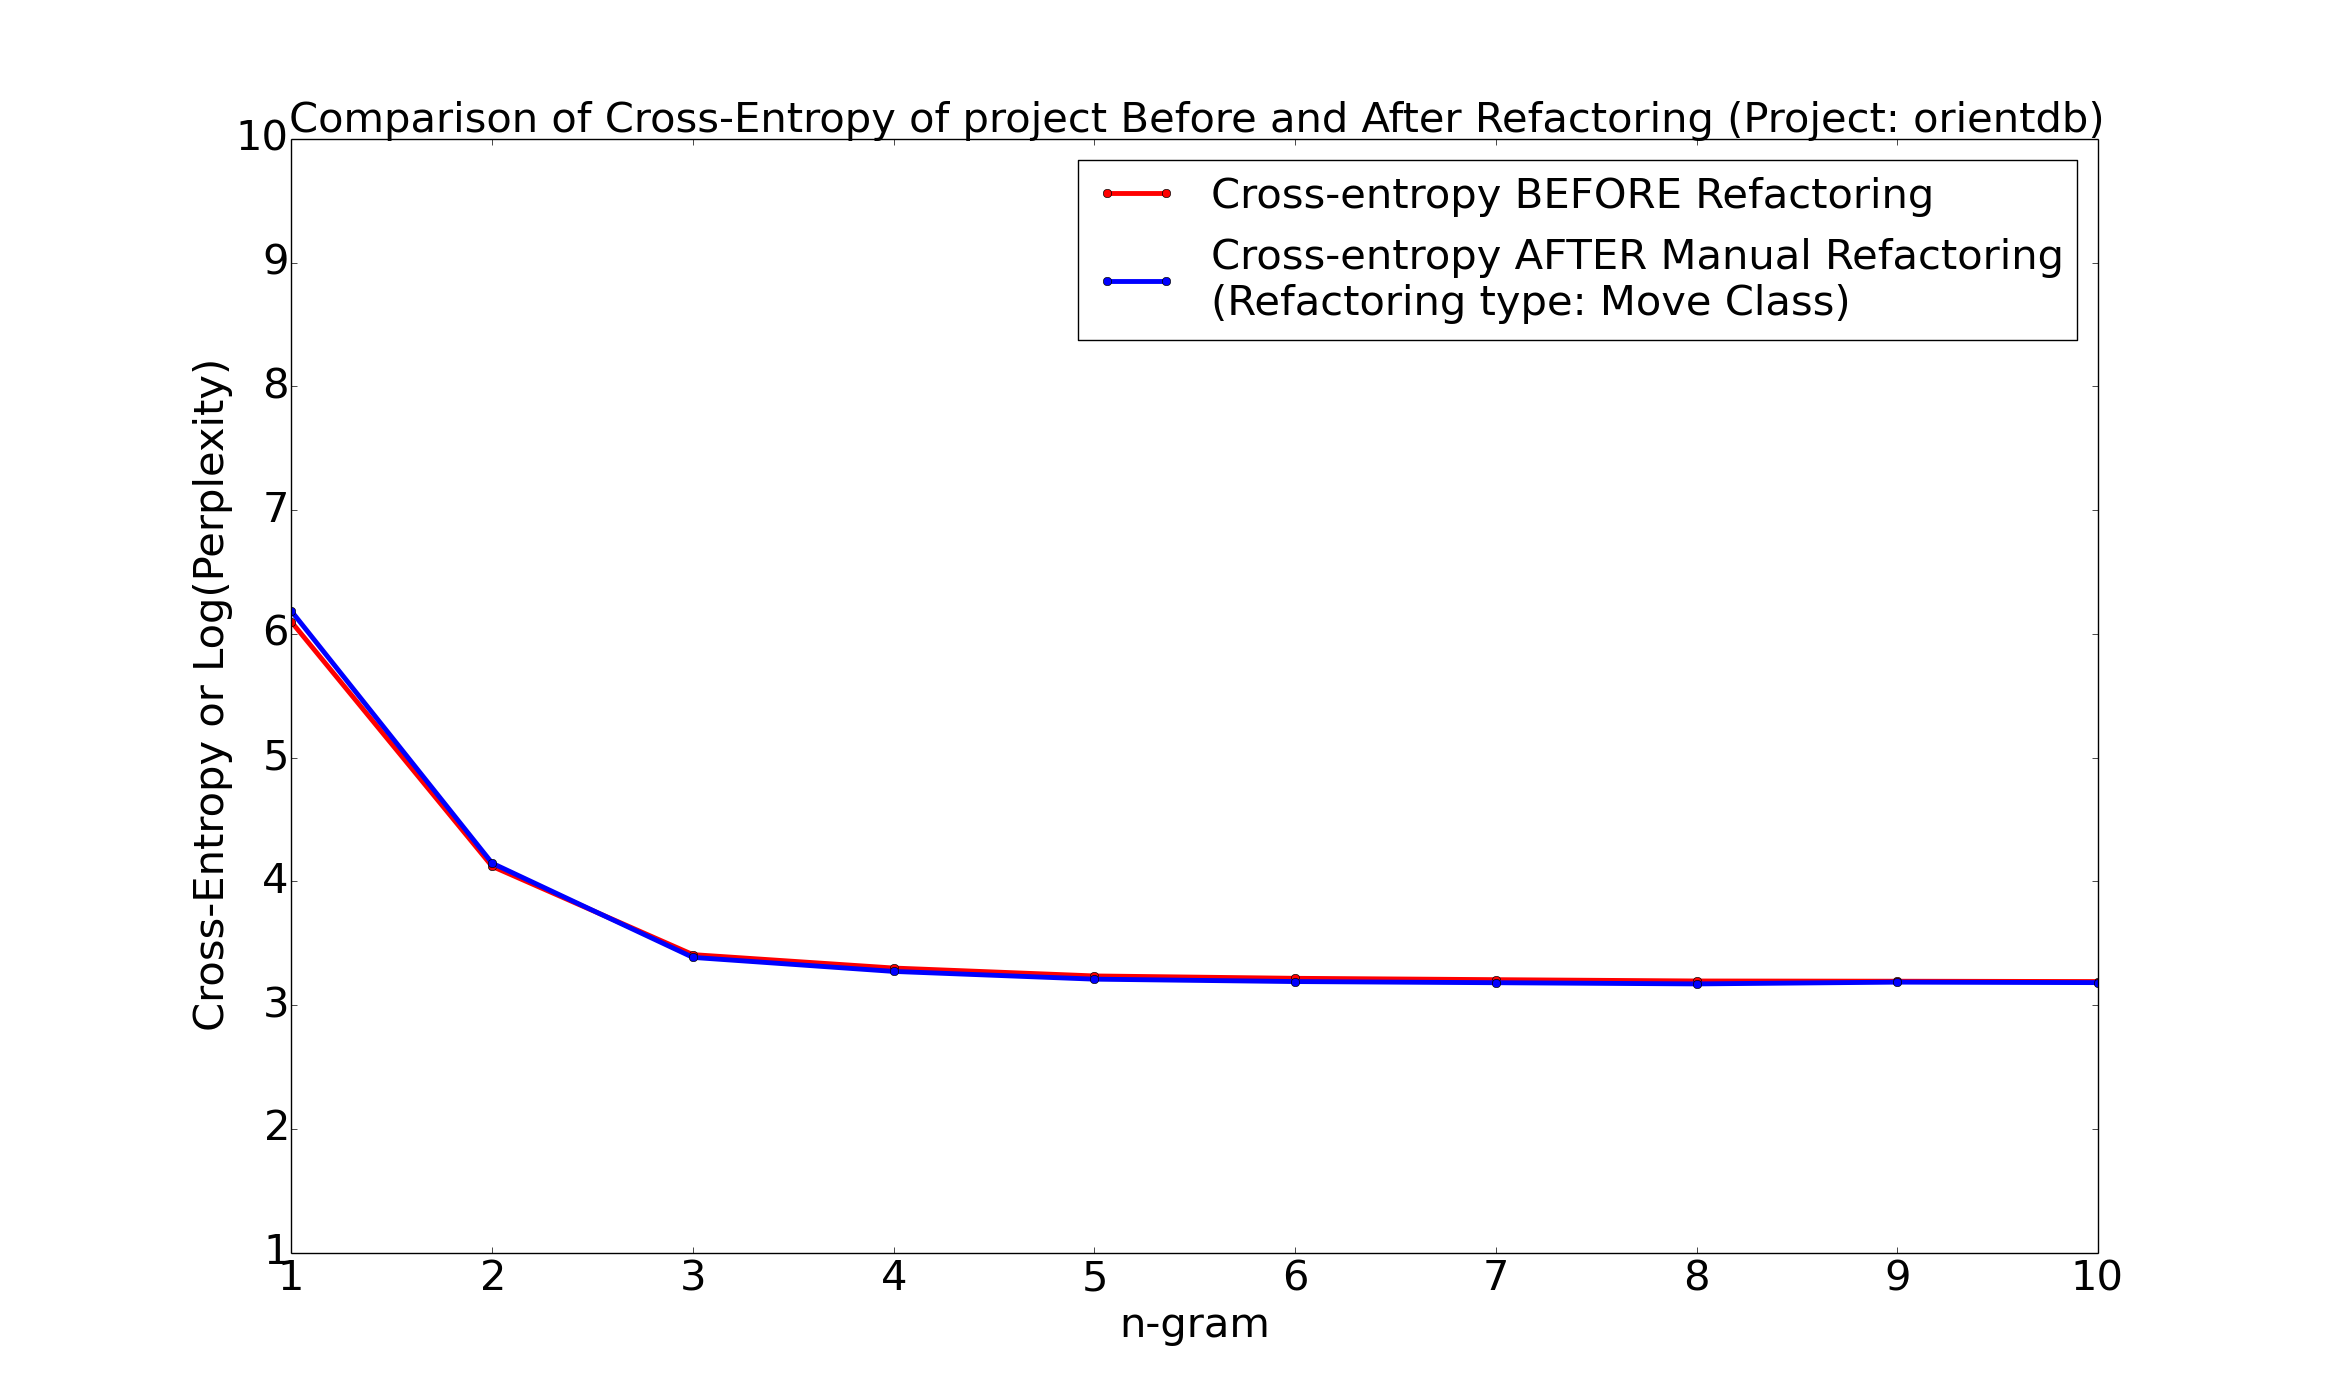
\includegraphics[width=150mm]{../Result/Refactoring_MoveClass/Plot/OrientDB.png}
\caption{Impact of Move Class Refactoring on project OrientDB}
\label{figure1}
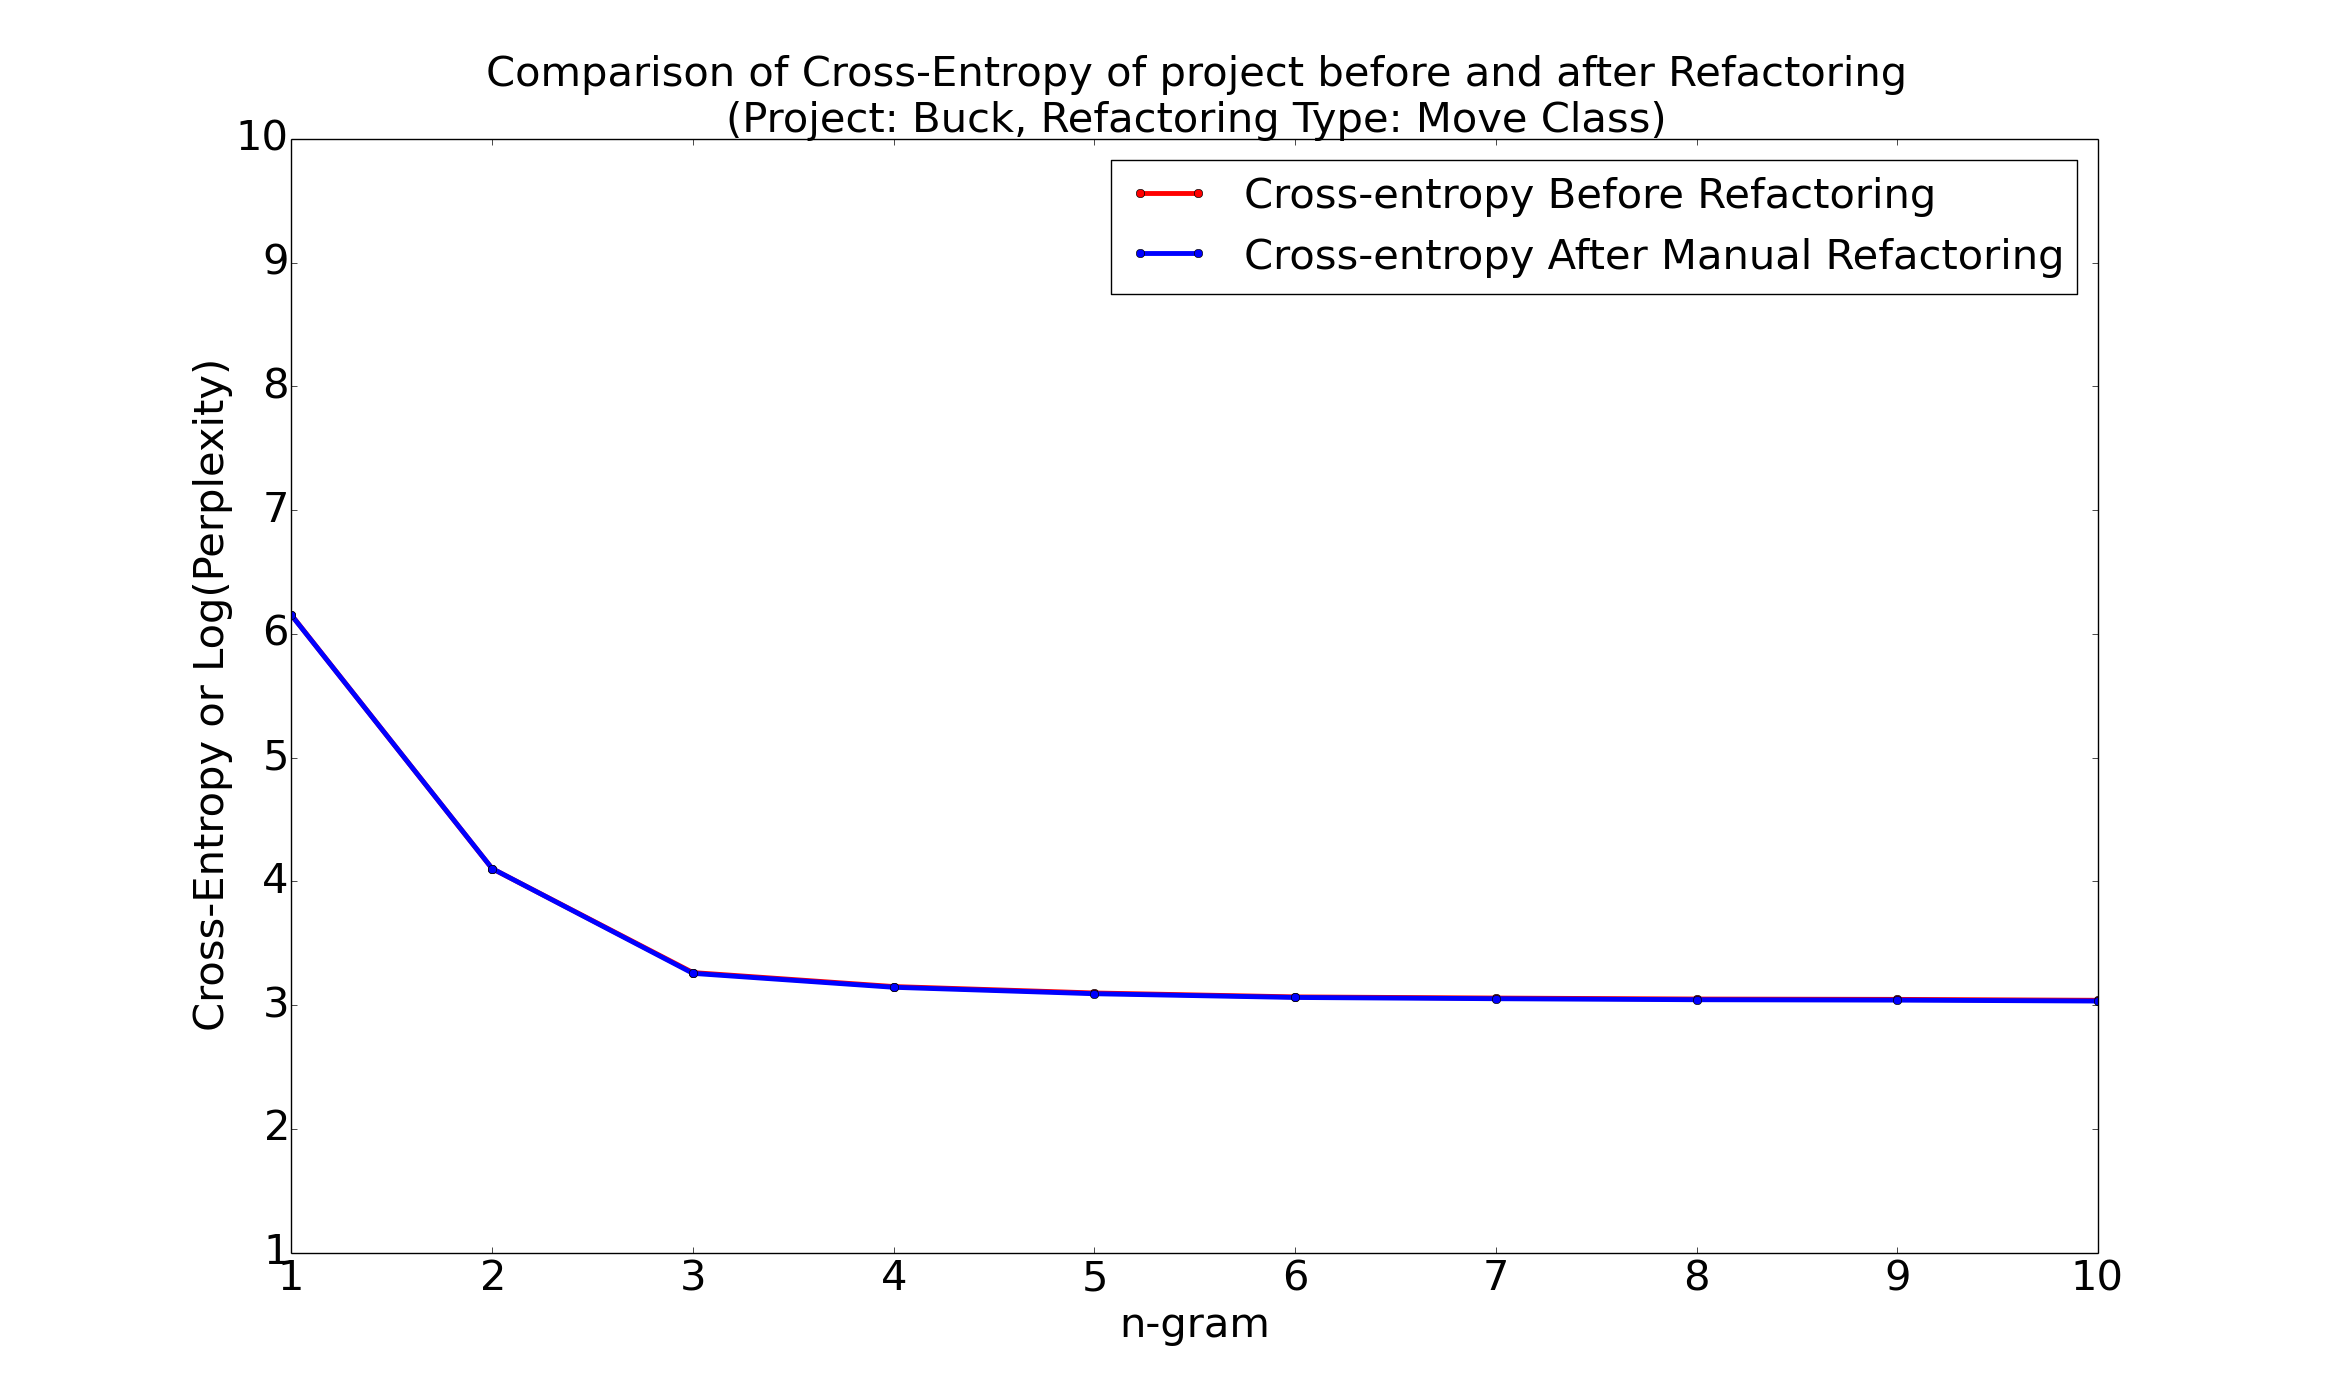
\includegraphics[width=150mm]{../Result/Refactoring_MoveClass/Plot/buck.png}
\caption{Impact of Move Class Refactoring on project Buck}
\label{figure2}
\end{figure*}

The fundamental purpose of performing refactoring is to make code more organized and maintainable. Intuitively we assume that making code more organized will reduce the value of cross-entropy, making it more regular and predictable. However, the result from our experiment proves that our intuition is not correct. Figure \ref{figure1} shows the result. From the plot it is vivid that for any vale of \textit{n} the cross-entropy of the project does not change after refactoring has been performed. Therefore, the overall perplexity remain same.

\subsection{Discussion} \label{ManualRefactDiscussion}
The result can be explained based on the count of tokens of each project. The count of total tokens, unique tokens and percentage of unique tokens are shown in Table \ref{SuammaryOrientDB}.

\begin{table*}[t]
\centering
\caption{Statistics for OrientDB}
\label{SuammaryOrientDB}
 \begin{tabular}{||c c c c||} 
 \hline
 Statistics & Before Refactoring & After Refactoring \\ [0.5ex] 
 \hline\hline
 Total Number of Tokens & 2152849 & 2154385 \\ 
 \hline
   Number of Unique Tokens & 35439 & 35480 \\
 \hline
	\% of Unique Tokens  & 0.0164614424885 & 0.0164687370178  \\ [1ex]  
 \hline
\end{tabular}
\end{table*}

The token level statistics of the project show that there is no significant change in the distribution of tokens before and after refactoring. Therefore, the cross-entropy remains same even if refactoring has been performed.

\noindent\fbox{%
   \parbox{\linewidth}{%
        \textbf{\textit{Refactoring does not effect the naturalness of source code. The cross-entropy of a project remains unchanged for any \textit{n-gram} before and after applying refactoring.}}
    }%
}

\section{Automated Refactoring} \label{ToolRefactoring}
\textit{RQ2. Tool-based or automated refactoring: Does automated refactoring change the naturalness?}

Many tools have been developed for making the task of refactoring easier, automated and less time consuming. From Section \ref{ReallRefactoring}  we conclude that manual refactoring does not change cross-entropy of a project with any level of significance. We investigate whether tool-based refactoring has any different effect on the cross-entropy. We use \textit{JDeodorant} \footnote{https://users.encs.concordia.ca/~nikolaos/jdeodorant/} plug-in of \textit{Eclipse} \footnote{http://www.eclipse.org/} to perform the refactorings.
\subsection{Finding}

\begin{figure*}[ht!]
\centering
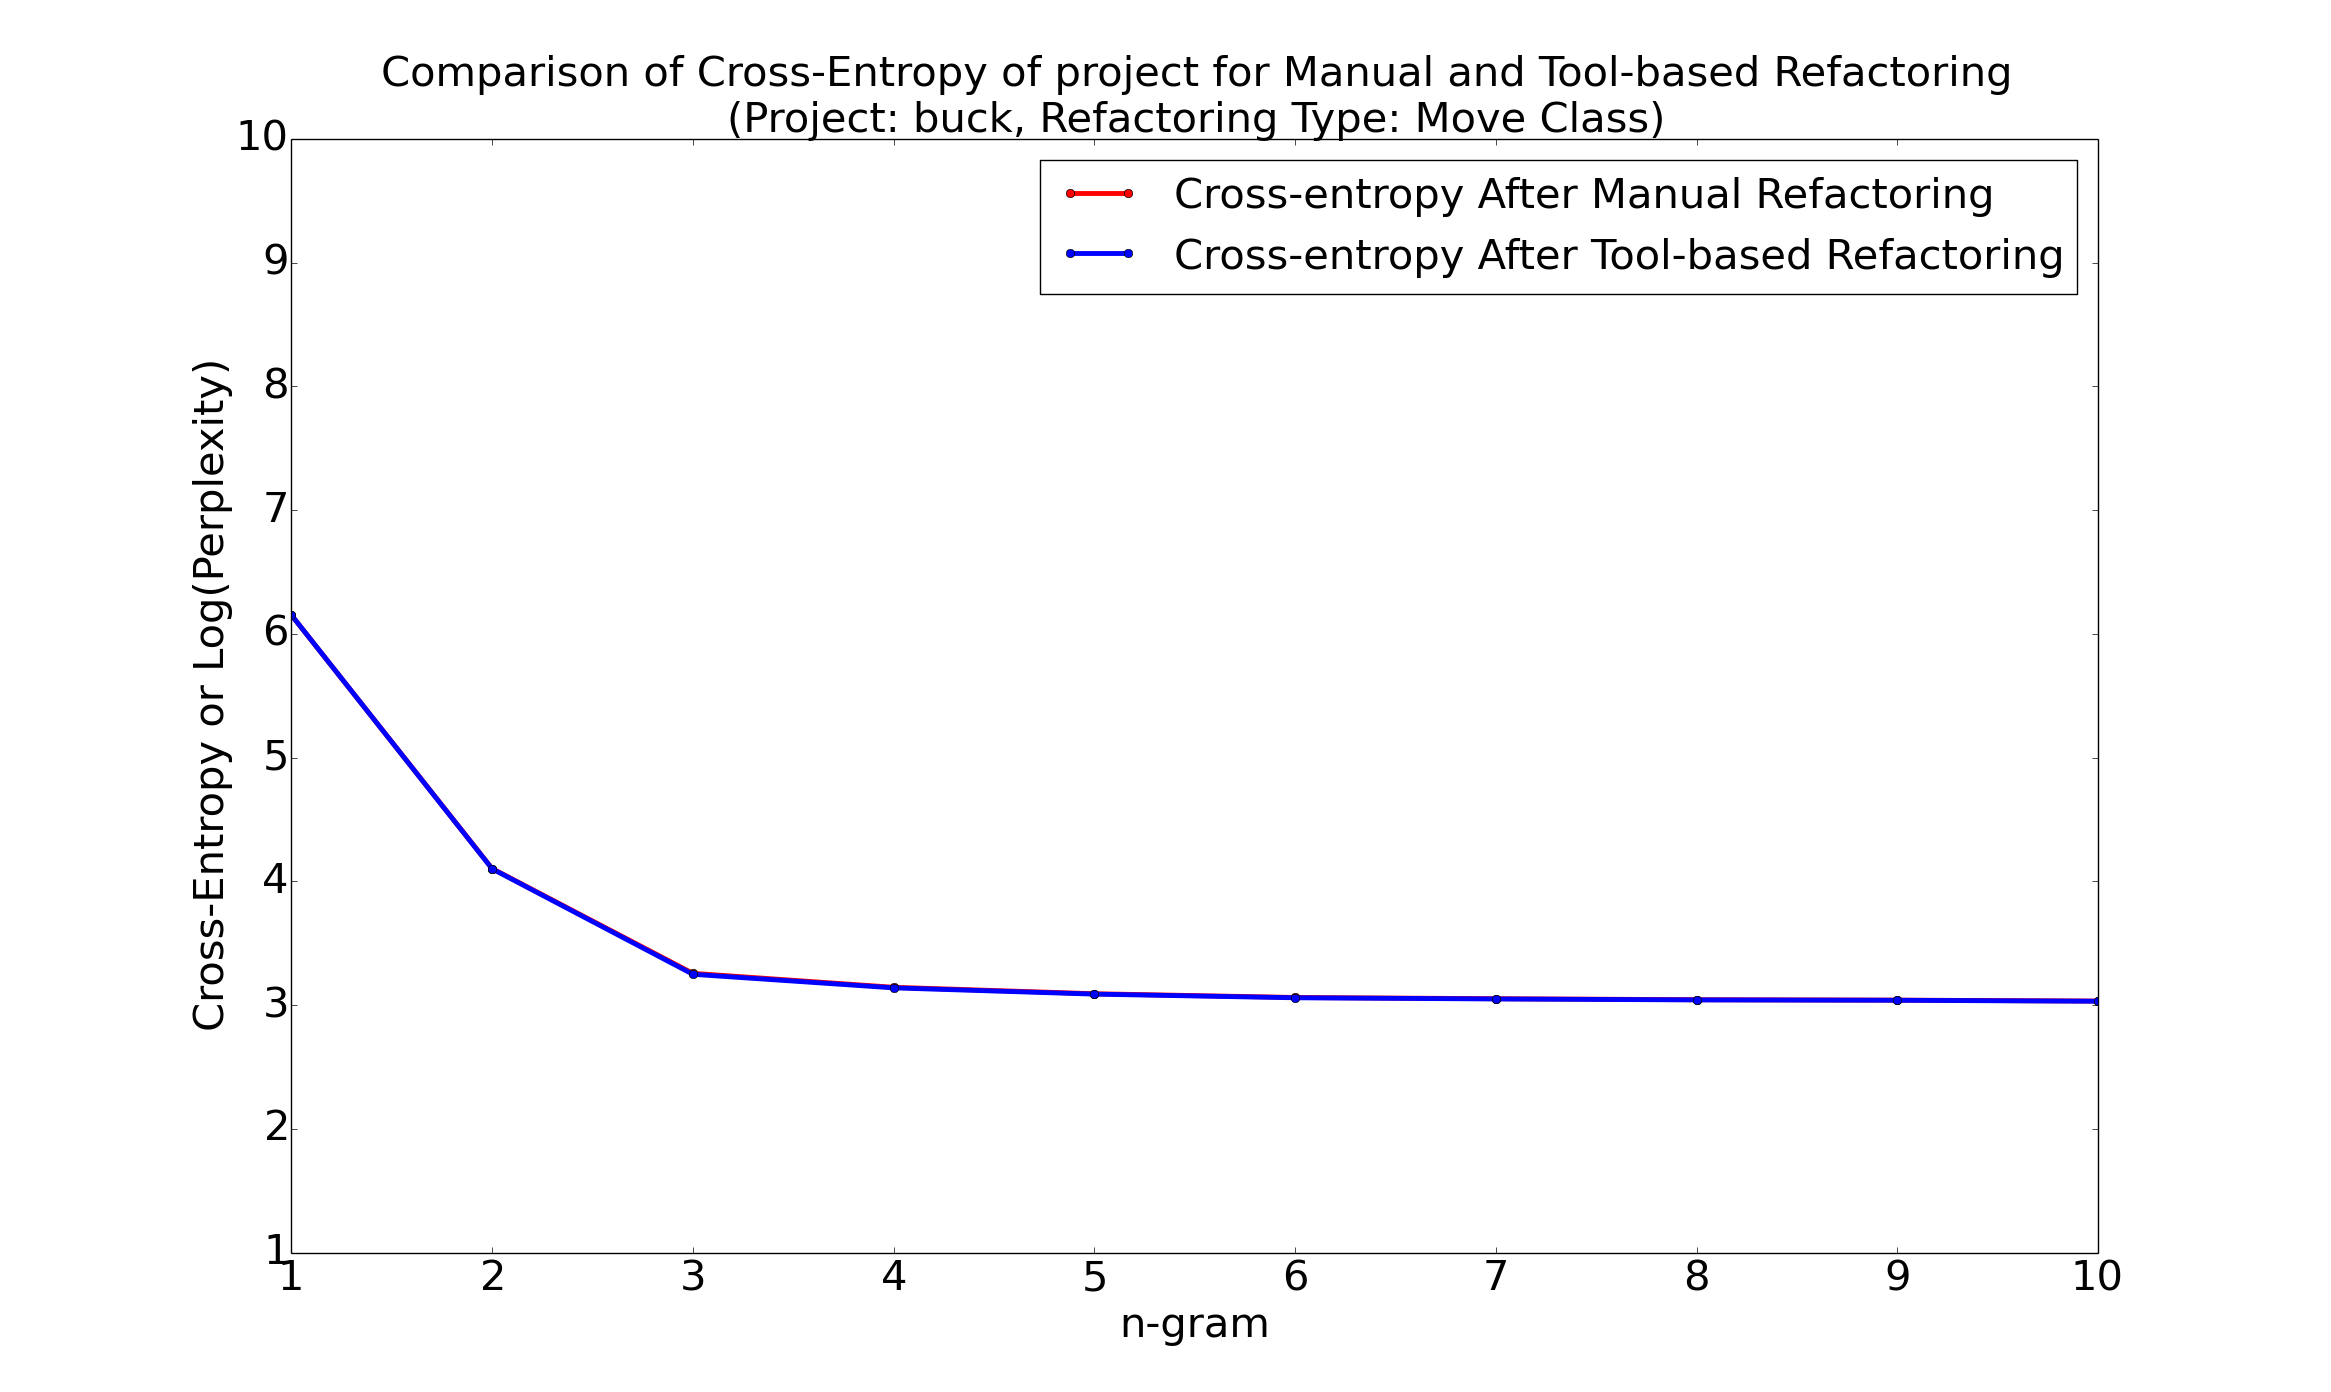
\includegraphics[width=150mm]{../Result/Refactoring_MoveClass/Plot/ManualVsTool_buck.png}
\caption{Comparison between tool-based and manual refactoring on project buck}
\label{figure3}
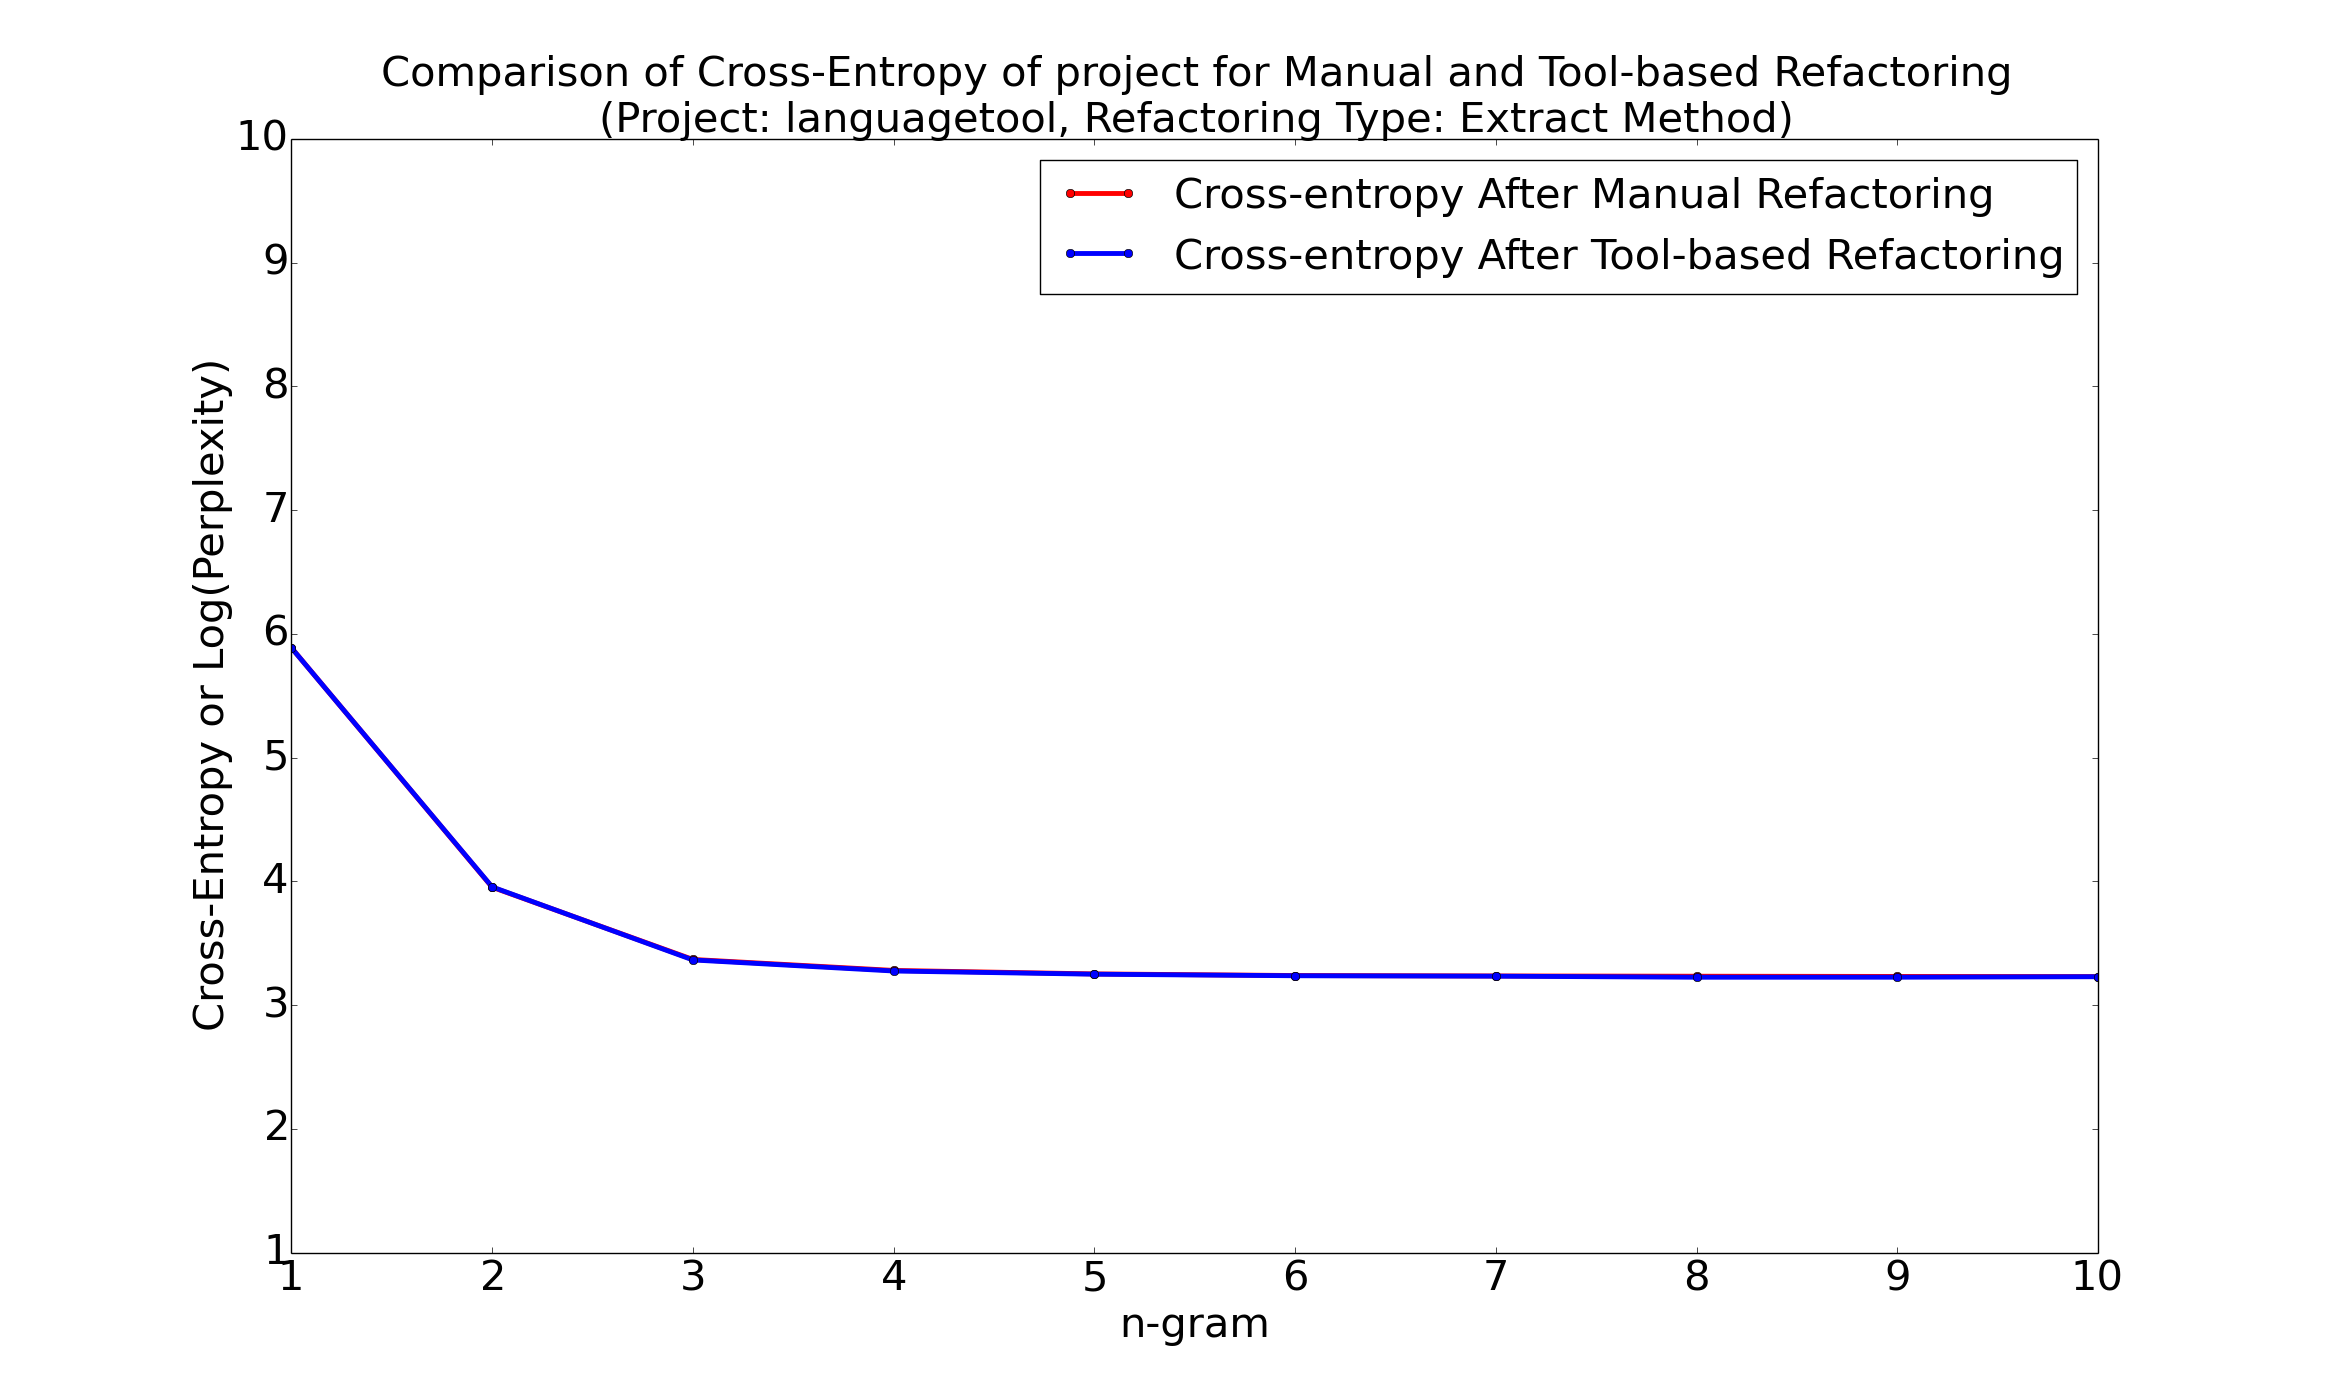
\includegraphics[width=150mm]{../Result/Refactoring_ExtractMethod/Plots/ToolVsManual_languagetool.png}
\caption{Comparison between tool-based and manual refactoring on project languagetool}
\label{figure4}
\end{figure*}

Figure \ref{figure3} and \ref{figure4} for show that the pattern of cross-entropy after manual and tool-based refactoring are exactly same. The curves have overlapped each other. Therefore, from linguistic point of view, refactoring using a tool does not contribute differently on the source code from the way that manual refactoring does.

\subsection{Discussion}

\begin{table*}[t]
\centering
\caption{Comparison of Statistics between manually and automated refactored code for project: languagetool}
\label{ComparisionLanguagetoll}
 \begin{tabular}{||c c c ||} 
 \hline
 Statistics & Manual Refactoring \\ [0.5ex] 
 \hline\hline
 Total Number of Tokens & 591189 & 605683 \\ 
 \hline
   Number of Unique Tokens & 32606 & 32639 \\
 \hline
	\% of Unique Tokens  & 0.0551532589409 & 0.0538879248716  \\ [1ex]  
 \hline
\end{tabular}
\end{table*}


\begin{table*}[t]
\centering
\caption{Comparison of Statistics between manually and automated refactored code for project: buck}
\label{ComparisionBuck}
 \begin{tabular}{||c c c ||} 
 \hline
 Statistics & Manual Refactoring & Tool-based Refactoring \\[0.5ex] 
 \hline\hline
 Total Number of Tokens & 1775290 & 1776152 \\ 
 \hline
   Number of Unique Tokens & 39906 & 39916  \\
 \hline
	\% of Unique Tokens  &  0.0224785809642 & 0.0224733018345 \\ [1ex]  
 \hline
\end{tabular}
\end{table*}

We can discuss the result in a same manner as we do in Section \ref{ManualRefactDiscussion}. The distribution of tokens play the most vital role in the cross-entropy value of the project. We can see from the statistics of tokens that the token distribution does not get affected differently even if we use tools (Table \ref{ComparisionLanguagetoll} and \ref{ComparisionBuck}).

\noindent\fbox{%
   \parbox{\linewidth}{%
        \textbf{\textit{Like manual refactoring, tool-based refactoring also do not have any significant impact on the cross-entropy of the project because of the fact that the distribution of tokens remain unchanged.}}
    }%
}



\section{Different types of Refactoring and Cross-entropy of source code}
\textit{RQ3, Types of refactoring: How do different types of refactoring affect the naturalness?}

We study four types of refactoring in this work:
\begin{itemize}
\item Extract Method
\item Inline Method
\item Move Class
\item Pull-up Method
\end{itemize}


\begin{figure*}[ht!]
\centering
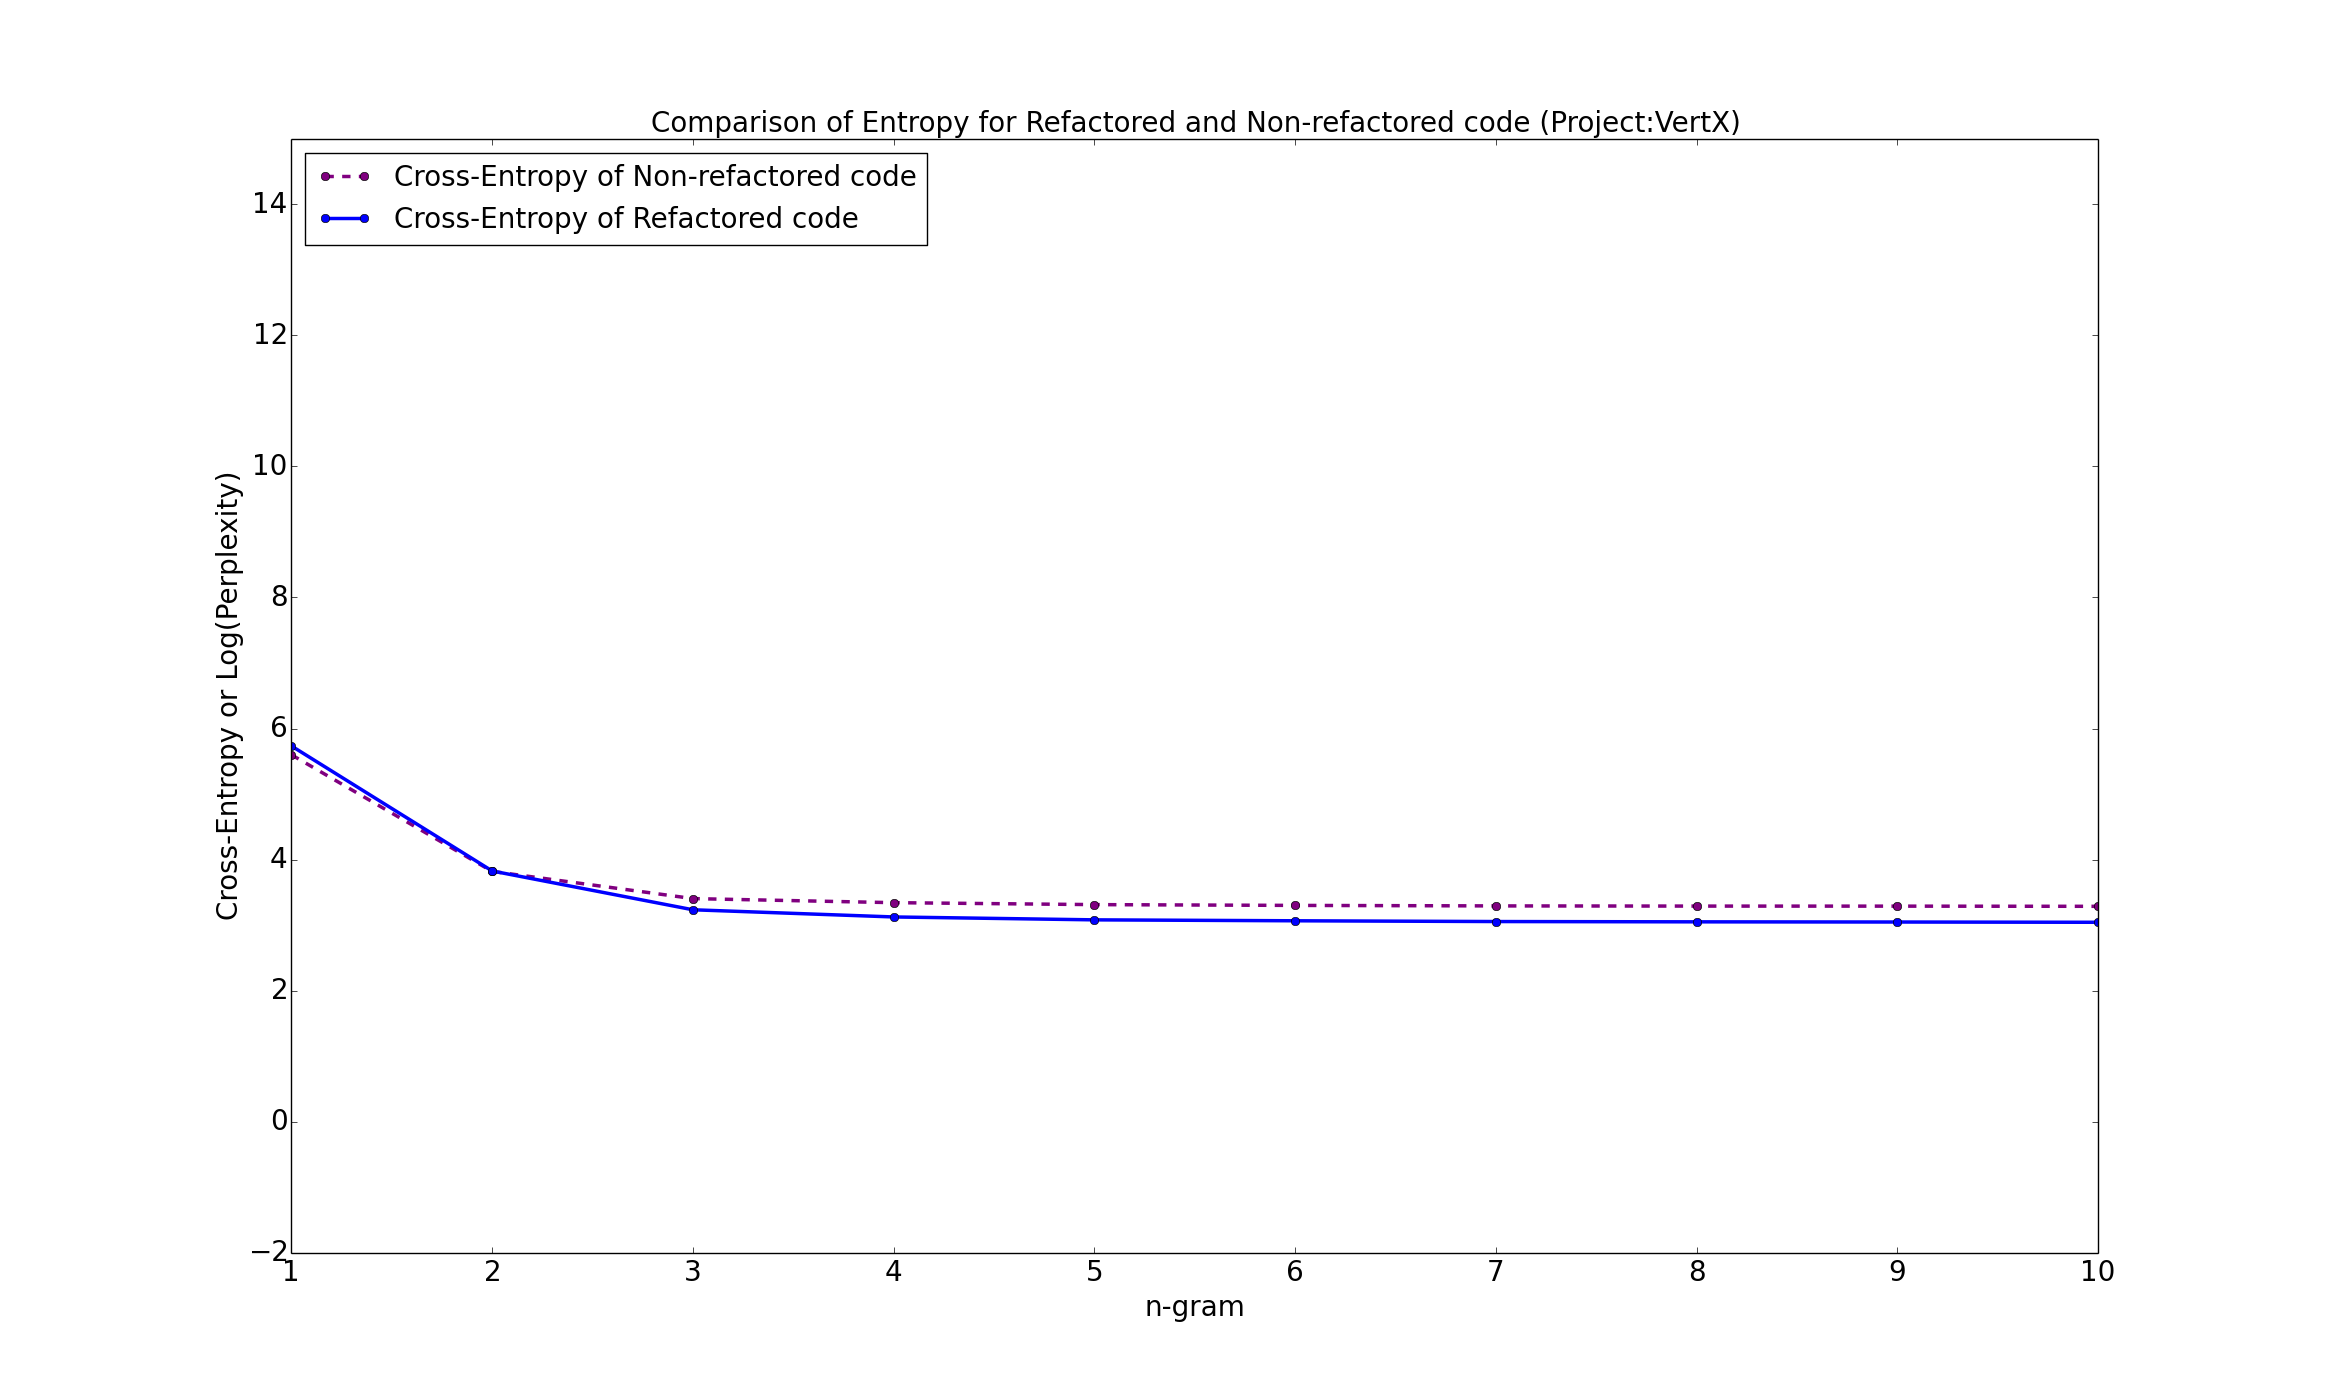
\includegraphics[width=150mm]{../Result/Refactoring_ExtractMethod/Plots/vertX.png}
\caption{Comparison of cross-entropy before and after refactoring on project Vert.X}
\label{figure5}
\end{figure*}
\begin{figure*}[ht!]
\centering
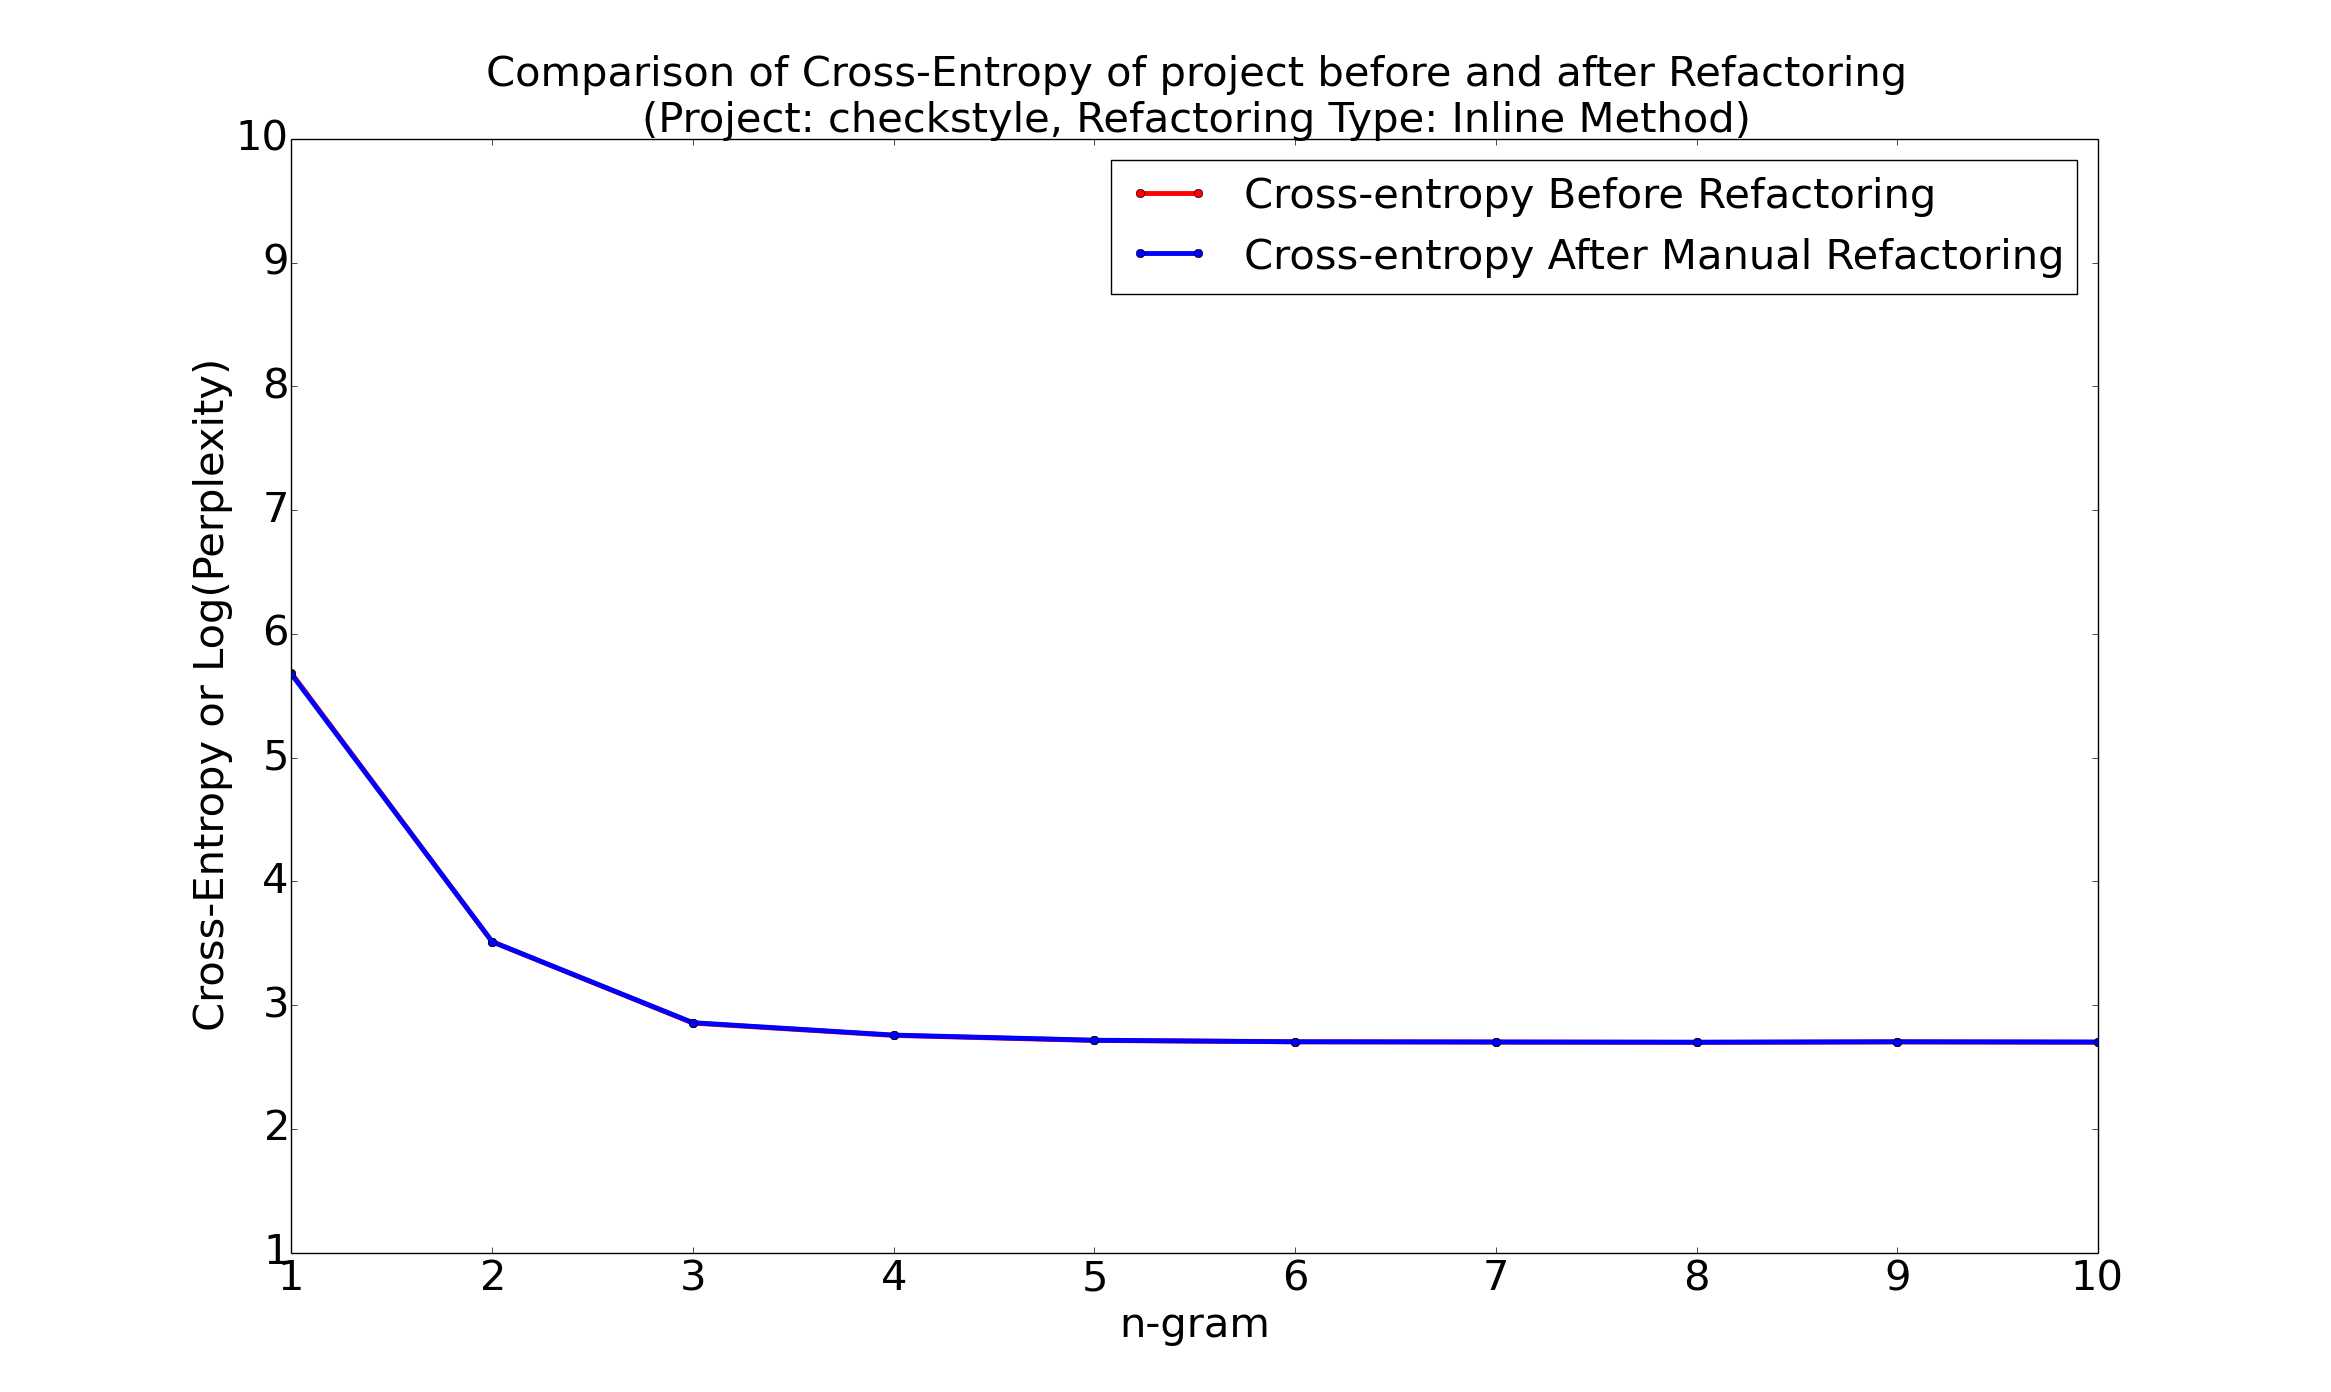
\includegraphics[width=150mm]{../Result/Refactoring_InlineMethod/Plots/checkstyle.png}
\caption{Comparison of cross-entropy before and after refactoring on project Checkstyle}
\label{figure6}
\end{figure*}
\begin{figure*}[ht!]
\centering
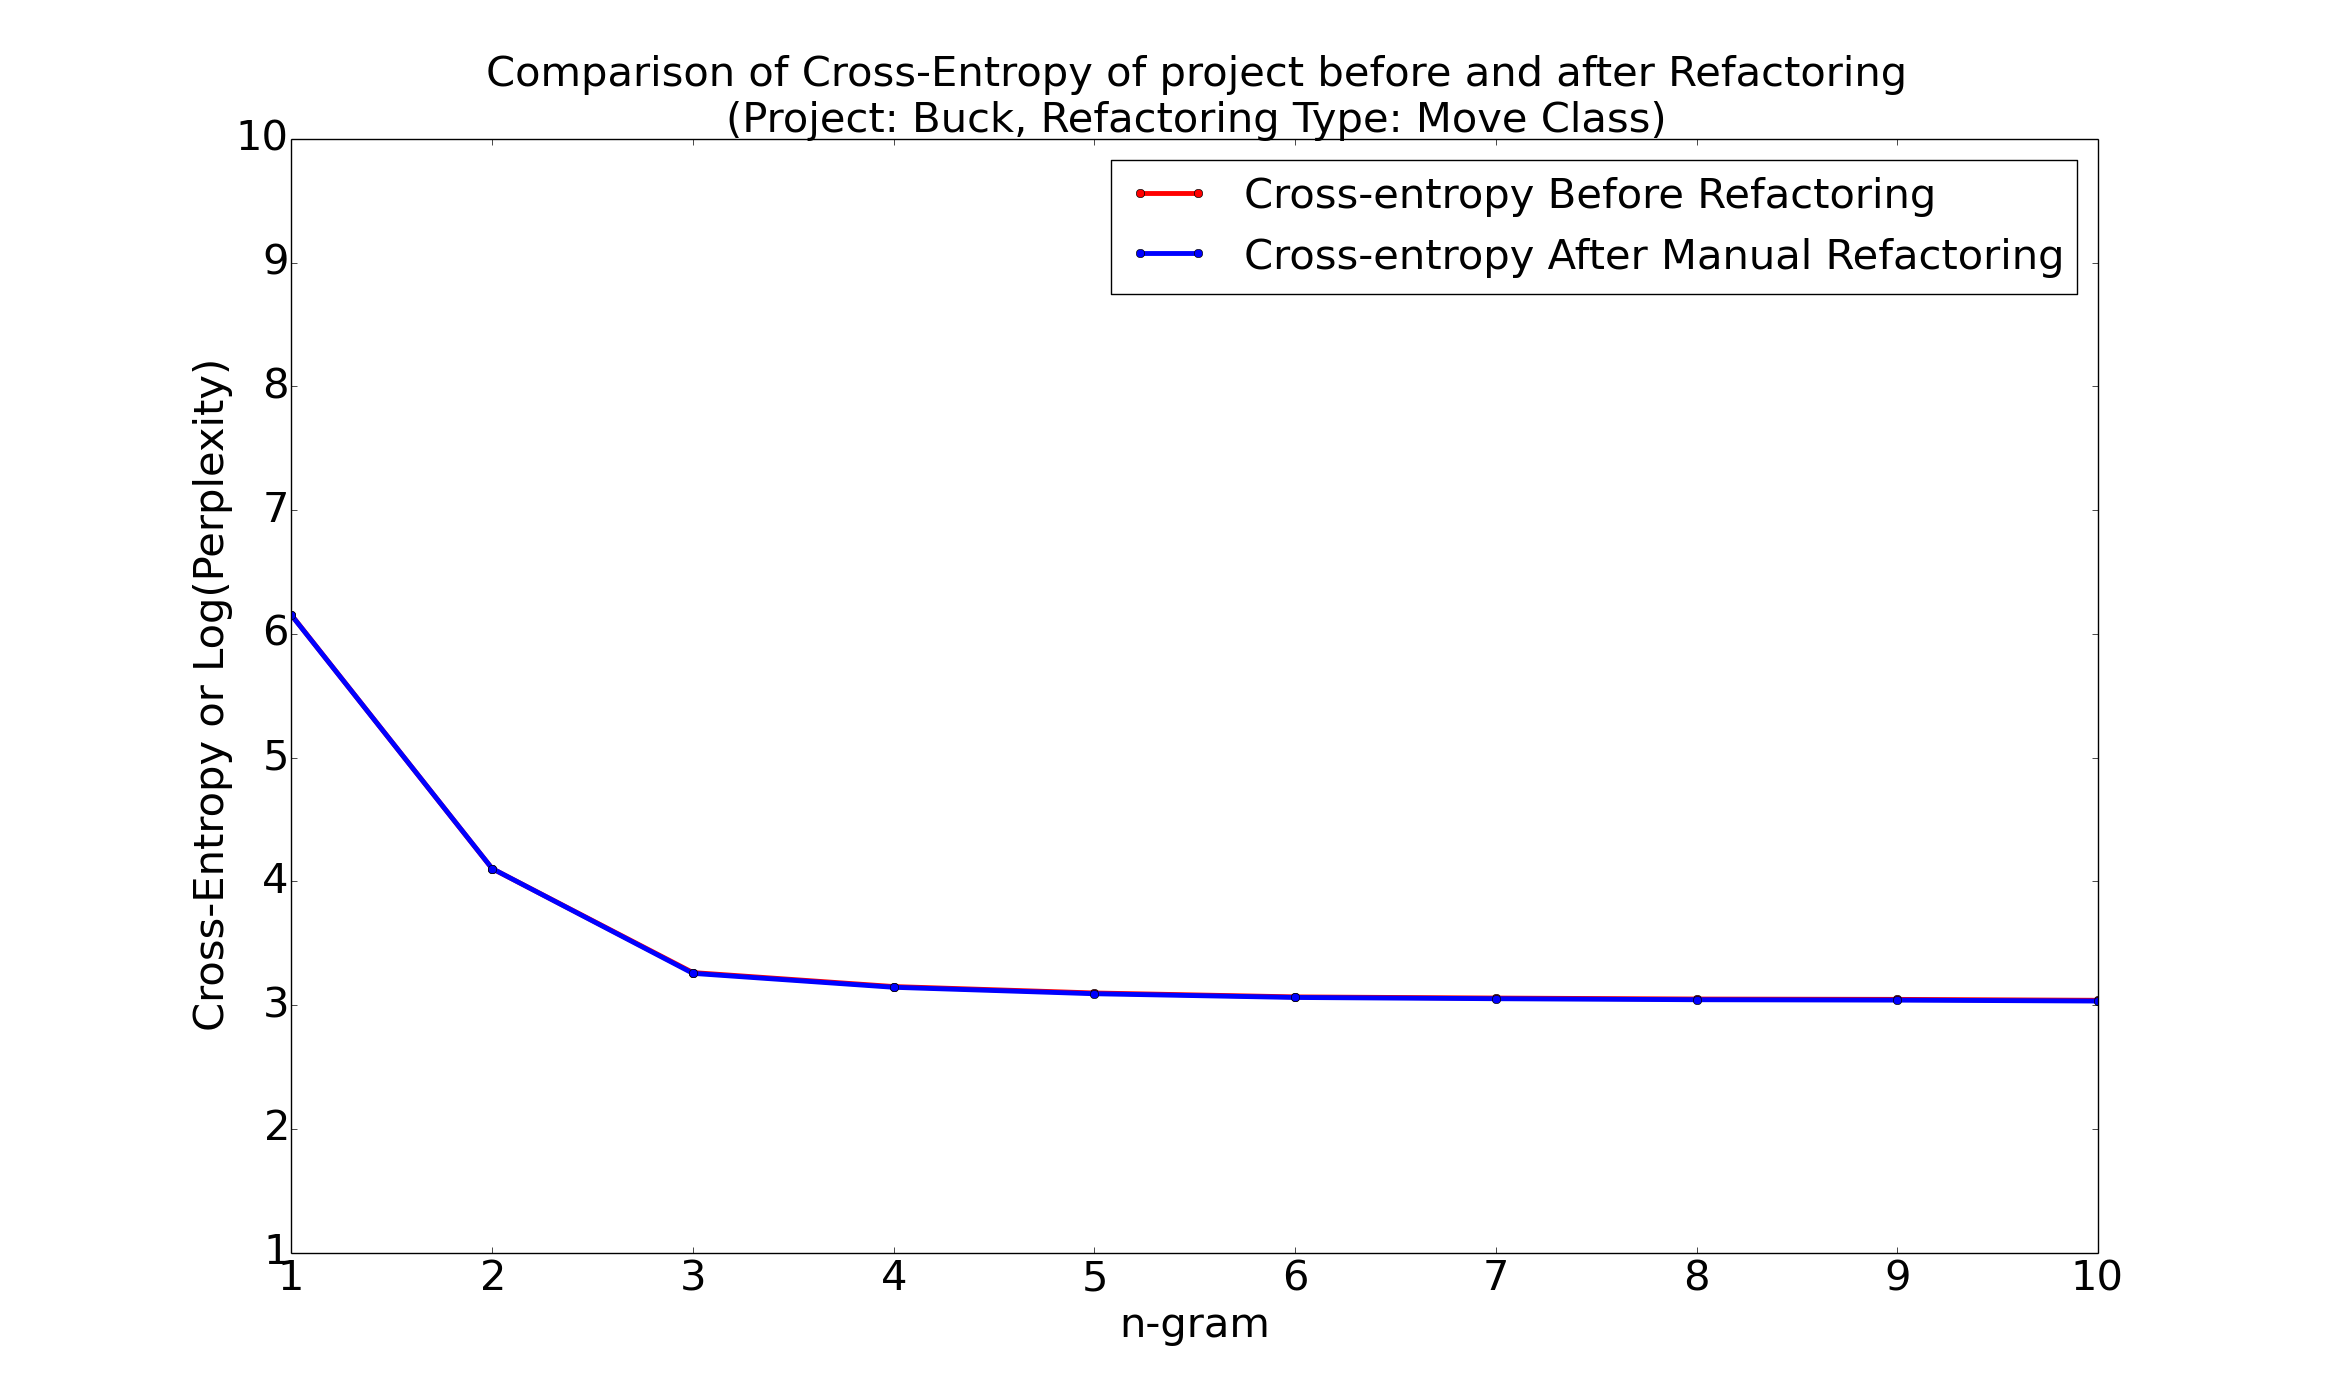
\includegraphics[width=150mm]{../Result/Refactoring_MoveClass/Plot/buck.png}
\caption{Comparison of cross-entropy before and after refactoring on project Buck}
\label{figure7}
\end{figure*}
\begin{figure*}[ht!]
\centering
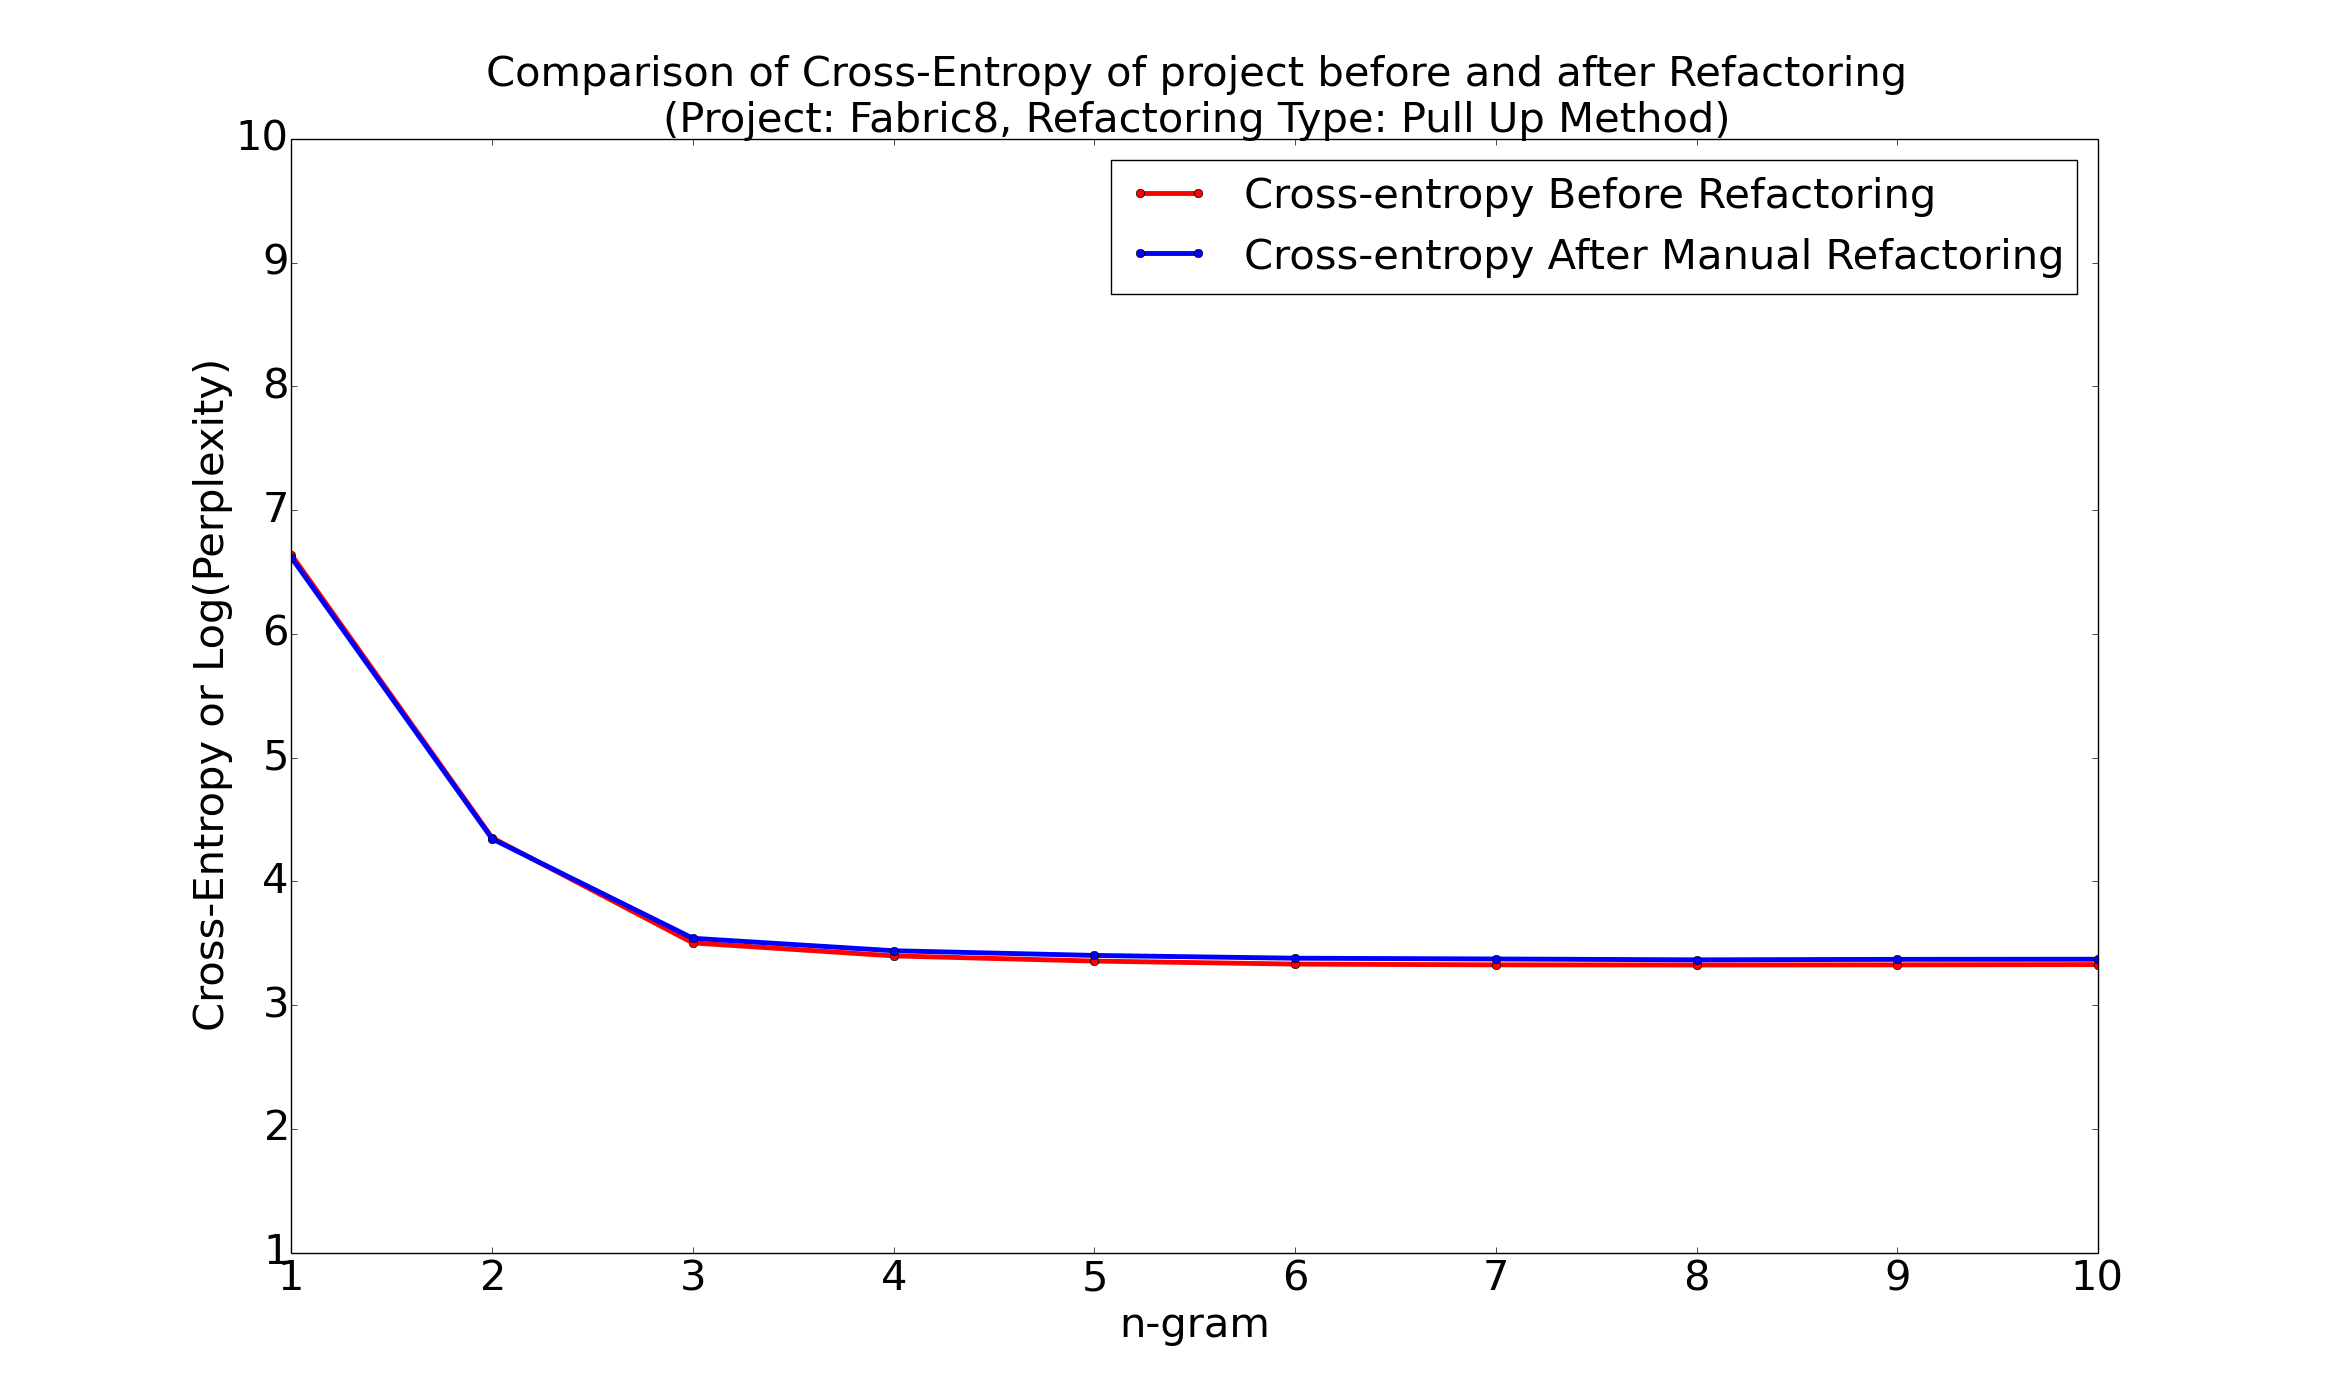
\includegraphics[width=150mm]{../Result/Refactoring_PullUpMethod/Plot/Fabric8.png}
\caption{Comparison of cross-entropy before and after refactoring on project Fabric8}
\label{figure8}
\end{figure*}


We observe the change in cross-entropy after performing each type of refactoring separately on different projects. The plots are shown in Figures \ref{figure5}, \ref{figure6}, \ref{figure7}, \ref{figure8}.



\subsection{Findings}

For the plots we see that the result of different refactoring types on different Java projects do not vary from each other. Over all cross-entropy does not get affected by any kind of refactoring.

\subsection{Discussion}

By definition of refactoring we keep the functionality of code same. Although we perform different types of refactoring, the over all distribution of tokens do not change significantly because of the fact that we just change the placement of tokens. This is the reason why refactoring does not impact the over all cross-entropy of the project.


\section{Conclusion}
In this work we show that refactoring do not play a role in the cross-entropy of projects. Cross-entropy of source code depend only on the distribution of tokens. Refactoring reorganizes code, it does not change features or functionalists. Because of this fact we hardly introduce new tokens in the code or remove tokens from the code. We essentially just change the placement of tokens to make sure that the code still does the same functions as it used to do before refactoring. This fundamental property of refactoring is proved by this study where we show that cross-entropy does not get affected by refactoring.

% An example of a floating figure using the graphicx package.
% Note that \label must occur AFTER (or within) \caption.
% For figures, \caption should occur after the \includegraphics.
% Note that IEEEtran v1.7 and later has special internal code that
% is designed to preserve the operation of \label within \caption
% even when the captionsoff option is in effect. However, because
% of issues like this, it may be the safest practice to put all your
% \label just after \caption rather than within \caption{}.
%
% Reminder: the "draftcls" or "draftclsnofoot", not "draft", class
% option should be used if it is desired that the figures are to be
% displayed while in draft mode.
%
%\begin{figure}[!t]
%\centering
%\includegraphics[width=2.5in]{myfigure}
% where an .eps filename suffix will be assumed under latex, 
% and a .pdf suffix will be assumed for pdflatex; or what has been declared
% via \DeclareGraphicsExtensions.
%\caption{Simulation results for the network.}
%\label{fig_sim}
%\end{figure}

% Note that the IEEE typically puts floats only at the top, even when this
% results in a large percentage of a column being occupied by floats.


% An example of a double column floating figure using two subfigures.
% (The subfig.sty package must be loaded for this to work.)
% The subfigure \label commands are set within each subfloat command,
% and the \label for the overall figure must come after \caption.
% \hfil is used as a separator to get equal spacing.
% Watch out that the combined width of all the subfigures on a 
% line do not exceed the text width or a line break will occur.
%
%\begin{figure*}[!t]
%\centering
%\subfloat[Case I]{\includegraphics[width=2.5in]{box}%
%\label{fig_first_case}}
%\hfil
%\subfloat[Case II]{\includegraphics[width=2.5in]{box}%
%\label{fig_second_case}}
%\caption{Simulation results for the network.}
%\label{fig_sim}
%\end{figure*}
%
% Note that often IEEE papers with subfigures do not employ subfigure
% captions (using the optional argument to \subfloat[]), but instead will
% reference/describe all of them (a), (b), etc., within the main caption.
% Be aware that for subfig.sty to generate the (a), (b), etc., subfigure
% labels, the optional argument to \subfloat must be present. If a
% subcaption is not desired, just leave its contents blank,
% e.g., \subfloat[].


% An example of a floating table. Note that, for IEEE style tables, the
% \caption command should come BEFORE the table and, given that table
% captions serve much like titles, are usually capitalized except for words
% such as a, an, and, as, at, but, by, for, in, nor, of, on, or, the, to
% and up, which are usually not capitalized unless they are the first or
% last word of the caption. Table text will default to \footnotesize as
% the IEEE normally uses this smaller font for tables.
% The \label must come after \caption as always.
%
%\begin{table}[!t]
%% increase table row spacing, adjust to taste
%\renewcommand{\arraystretch}{1.3}
% if using array.sty, it might be a good idea to tweak the value of
% \extrarowheight as needed to properly center the text within the cells
%\caption{An Example of a Table}
%\label{table_example}
%\centering
%% Some packages, such as MDW tools, offer better commands for making tables
%% than the plain LaTeX2e tabular which is used here.
%\begin{tabular}{|c||c|}
%\hline
%One & Two\\
%\hline
%Three & Four\\
%\hline
%\end{tabular}
%\end{table}


% Note that the IEEE does not put floats in the very first column
% - or typically anywhere on the first page for that matter. Also,
% in-text middle ("here") positioning is typically not used, but it
% is allowed and encouraged for Computer Society conferences (but
% not Computer Society journals). Most IEEE journals/conferences use
% top floats exclusively. 
% Note that, LaTeX2e, unlike IEEE journals/conferences, places
% footnotes above bottom floats. This can be corrected via the
% \fnbelowfloat command of the stfloats package.





% conference papers do not normally have an appendix


% use section* for acknowledgment
%\section*{Acknowledgment}


%The authors would like to thank...





% trigger a \newpage just before the given reference
% number - used to balance the columns on the last page
% adjust value as needed - may need to be readjusted if
% the document is modified later
%\IEEEtriggeratref{8}
% The "triggered" command can be changed if desired:
%\IEEEtriggercmd{\enlargethispage{-5in}}

% references section

% can use a bibliography generated by BibTeX as a .bbl file
% BibTeX documentation can be easily obtained at:
% http://mirror.ctan.org/biblio/bibtex/contrib/doc/
% The IEEEtran BibTeX style support page is at:
% http://www.michaelshell.org/tex/ieeetran/bibtex/
%\bibliographystyle{IEEEtran}
% argument is your BibTeX string definitions and bibliography database(s)
%\bibliography{IEEEabrv,../bib/paper}
%
% <OR> manually copy in the resultant .bbl file
% set second argument of \begin to the number of references
% (used to reserve space for the reference number labels box)
\begin{thebibliography}{}

\bibitem{Brown}
Peter F. Brown, John Cocke, Stephen A. Della Pietra, Vincent J. Della Pietra, Fredrick Jelinek, John D. Lafferty, Robert L. Mercer, and Paul S. Roossin. 1990. A statistical approach to machine translation. Comput. Linguist. 16, 2 (June 1990), 79-85. 

\bibitem{Ray}
Baishakhi Ray, Vincent Hellendoorn, Saheel Godhane, Zhaopeng Tu, Alberto Bacchelli, and Premkumar Devanbu. 2016. On the "naturalness" of buggy code. In Proceedings of the 38th International Conference on Software Engineering (ICSE '16). ACM, New York, NY, USA, 428-439. DOI=http://dx.doi.org/10.1145/2884781.2884848 

\bibitem{Hindle}
Abram Hindle, Earl T. Barr, Zhendong Su, Mark Gabel, and Premkumar Devanbu. 2012. On the naturalness of software. In Proceedings of the 34th International Conference on Software Engineering (ICSE '12). IEEE Press, Piscataway, NJ, USA, 837-847.

\bibitem{Murphy}
Emerson Murphy-Hill, Chris Parnin, and Andrew P. Black. 2009. How we refactor, and how we know it. In Proceedings of the 31st International Conference on Software Engineering (ICSE '09). IEEE Computer Society, Washington, DC, USA, 287-297. DOI=10.1109/ICSE.2009.5070529 http://dx.doi.org/10.1109/ICSE.2009.5070529

\bibitem{Tu}
Zhaopeng Tu, Zhendong Su, and Premkumar Devanbu. 2014. On the localness of software. In Proceedings of the 22nd ACM SIGSOFT International Symposium on Foundations of Software Engineering (FSE 2014). ACM, New York, NY, USA, 269-280. DOI: http://dx.doi.org/10.1145/2635868.2635875

\bibitem{Silva}
Danilo Silva, Nikolaos Tsantalis, and Marco Tulio Valente. 2016. Why We Refactor? Confessions of GitHub Contributors. In Proceedings of the 24th ACM SIGSOFT International Symposium on the Foundations of Software Engineering (FSE'2016), Seattle, WA.

\bibitem{GailMurphy}
Gail C. Murphy, Mik Kersten, and Leah Findlater. 2006. How Are Java Software Developers Using the Eclipse IDE?. IEEE Softw. 23, 4 (July 2006), 76-83. DOI=http://dx.doi.org/10.1109/MS.2006.105

\bibitem{Davood}
Davood Mazinanian, Nikolaos Tsantalis, Raphael Stein, and Zackary Valenta. 2016. JDeodorant: Clone Refactoring. pp. 613-616, 38th International Conference on Software Engineering (ICSE'2016), Formal Tool Demonstration Session, Austin, Texas, USA.

\bibitem{Zibran}
M. F. Zibran and C. K. Roy. 2013. Conflict-aware Optimal Scheduling of Code Clone Refactoring. IET Software, Volume 7(3), June 2013, pp. 167-186.

\bibitem{Mondal}
M. Mondal, C. K. Roy and K. A. Schneider, "Automatic Identification of Important Clones for Refactoring and Tracking," Source Code Analysis and Manipulation (SCAM), 2014 IEEE 14th International Working Conference on, Victoria, BC, 2014, pp. 11-20.
doi: 10.1109/SCAM.2014.11

\bibitem{Fokaefs}
Marios Fokaefs, Nikolaos Tsantalis, Eleni Stroulia, and Alexander Chatzigeorgiou. 2012. Identification and application of Extract Class refactorings in object-oriented systems. J. Syst. Softw. 85, 10 (October 2012), 2241-2260. DOI=http://dx.doi.org/10.1016/j.jss.2012.04.013 

\bibitem{Opdyke}
W. F. Opdyke. 1992. Refactoring object-oriented frameworks. PhD thesis, University of Illinois at Urbana-Champaign, IL, USA.

\bibitem{Tsantalis}
Nikolaos Tsantalis and Alexander Chatzigeorgiou. 2010. Identification of refactoring opportunities introducing polymorphism. J. Syst. Softw. 83, 3 (March 2010), 391-404. DOI=http://dx.doi.org/10.1016/j.jss.2009.09.017

\bibitem{Koehn}
Philipp Koehn. 2009. Statistical machine translation. Chapter 7, Cambridge University Press.

\bibitem{Jones}
K. Sparck Jones. 1994. Natural language processing: a historical review. Current Issues in Computational Linguistics: in Honour of Don Walker (Ed Zampolli, Calzolari and Palmer), Amsterdam.

\bibitem{Campbell}
Joshua Charles Campbell, Abram Hindle, and José Nelson Amaral. 2014. Syntax errors just aren't natural: improving error reporting with language models. In Proceedings of the 11th Working Conference on Mining Software Repositories (MSR 2014). ACM, New York, NY, USA, 252-261. DOI: http://dx.doi.org/10.1145/2597073.2597102

\bibitem{Zhang}
Y. F. Zhang, Q. F. Zhang and R. H. Yu. 2010. Markov property of Markov chains and its test. International Conference on Machine Learning and Cybernetics, Qingdao, 2010, pp. 1864-1867. doi: 10.1109/ICMLC.2010.5580952

\bibitem{NikolaosTsantalis}
Nikolaos Tsantalis, Victor Guana, Eleni Stroulia, and Abram Hindle. 2013. A multidimensional empirical study on refactoring activity. In Proceedings of the 2013 Conference of the Center for Advanced Studies on Collaborative Research (CASCON '13). IBM Corp., Riverton, NJ, USA, 132-146. 

\end{thebibliography}




% that's all folks
\end{document}


